% Options for packages loaded elsewhere
\PassOptionsToPackage{unicode}{hyperref}
\PassOptionsToPackage{hyphens}{url}
%
\documentclass[
]{article}
\usepackage{amsmath,amssymb}
\usepackage{lmodern}
\usepackage{ifxetex,ifluatex}
\ifnum 0\ifxetex 1\fi\ifluatex 1\fi=0 % if pdftex
  \usepackage[T1]{fontenc}
  \usepackage[utf8]{inputenc}
  \usepackage{textcomp} % provide euro and other symbols
\else % if luatex or xetex
  \usepackage{unicode-math}
  \defaultfontfeatures{Scale=MatchLowercase}
  \defaultfontfeatures[\rmfamily]{Ligatures=TeX,Scale=1}
\fi
% Use upquote if available, for straight quotes in verbatim environments
\IfFileExists{upquote.sty}{\usepackage{upquote}}{}
\IfFileExists{microtype.sty}{% use microtype if available
  \usepackage[]{microtype}
  \UseMicrotypeSet[protrusion]{basicmath} % disable protrusion for tt fonts
}{}
\makeatletter
\@ifundefined{KOMAClassName}{% if non-KOMA class
  \IfFileExists{parskip.sty}{%
    \usepackage{parskip}
  }{% else
    \setlength{\parindent}{0pt}
    \setlength{\parskip}{6pt plus 2pt minus 1pt}}
}{% if KOMA class
  \KOMAoptions{parskip=half}}
\makeatother
\usepackage{xcolor}
\IfFileExists{xurl.sty}{\usepackage{xurl}}{} % add URL line breaks if available
\IfFileExists{bookmark.sty}{\usepackage{bookmark}}{\usepackage{hyperref}}
\hypersetup{
  pdftitle={Determining Authentic News Articles using Machine Learning},
  pdfauthor={Uday Adusumilli},
  hidelinks,
  pdfcreator={LaTeX via pandoc}}
\urlstyle{same} % disable monospaced font for URLs
\usepackage[margin=1in]{geometry}
\usepackage{color}
\usepackage{fancyvrb}
\newcommand{\VerbBar}{|}
\newcommand{\VERB}{\Verb[commandchars=\\\{\}]}
\DefineVerbatimEnvironment{Highlighting}{Verbatim}{commandchars=\\\{\}}
% Add ',fontsize=\small' for more characters per line
\usepackage{framed}
\definecolor{shadecolor}{RGB}{248,248,248}
\newenvironment{Shaded}{\begin{snugshade}}{\end{snugshade}}
\newcommand{\AlertTok}[1]{\textcolor[rgb]{0.94,0.16,0.16}{#1}}
\newcommand{\AnnotationTok}[1]{\textcolor[rgb]{0.56,0.35,0.01}{\textbf{\textit{#1}}}}
\newcommand{\AttributeTok}[1]{\textcolor[rgb]{0.77,0.63,0.00}{#1}}
\newcommand{\BaseNTok}[1]{\textcolor[rgb]{0.00,0.00,0.81}{#1}}
\newcommand{\BuiltInTok}[1]{#1}
\newcommand{\CharTok}[1]{\textcolor[rgb]{0.31,0.60,0.02}{#1}}
\newcommand{\CommentTok}[1]{\textcolor[rgb]{0.56,0.35,0.01}{\textit{#1}}}
\newcommand{\CommentVarTok}[1]{\textcolor[rgb]{0.56,0.35,0.01}{\textbf{\textit{#1}}}}
\newcommand{\ConstantTok}[1]{\textcolor[rgb]{0.00,0.00,0.00}{#1}}
\newcommand{\ControlFlowTok}[1]{\textcolor[rgb]{0.13,0.29,0.53}{\textbf{#1}}}
\newcommand{\DataTypeTok}[1]{\textcolor[rgb]{0.13,0.29,0.53}{#1}}
\newcommand{\DecValTok}[1]{\textcolor[rgb]{0.00,0.00,0.81}{#1}}
\newcommand{\DocumentationTok}[1]{\textcolor[rgb]{0.56,0.35,0.01}{\textbf{\textit{#1}}}}
\newcommand{\ErrorTok}[1]{\textcolor[rgb]{0.64,0.00,0.00}{\textbf{#1}}}
\newcommand{\ExtensionTok}[1]{#1}
\newcommand{\FloatTok}[1]{\textcolor[rgb]{0.00,0.00,0.81}{#1}}
\newcommand{\FunctionTok}[1]{\textcolor[rgb]{0.00,0.00,0.00}{#1}}
\newcommand{\ImportTok}[1]{#1}
\newcommand{\InformationTok}[1]{\textcolor[rgb]{0.56,0.35,0.01}{\textbf{\textit{#1}}}}
\newcommand{\KeywordTok}[1]{\textcolor[rgb]{0.13,0.29,0.53}{\textbf{#1}}}
\newcommand{\NormalTok}[1]{#1}
\newcommand{\OperatorTok}[1]{\textcolor[rgb]{0.81,0.36,0.00}{\textbf{#1}}}
\newcommand{\OtherTok}[1]{\textcolor[rgb]{0.56,0.35,0.01}{#1}}
\newcommand{\PreprocessorTok}[1]{\textcolor[rgb]{0.56,0.35,0.01}{\textit{#1}}}
\newcommand{\RegionMarkerTok}[1]{#1}
\newcommand{\SpecialCharTok}[1]{\textcolor[rgb]{0.00,0.00,0.00}{#1}}
\newcommand{\SpecialStringTok}[1]{\textcolor[rgb]{0.31,0.60,0.02}{#1}}
\newcommand{\StringTok}[1]{\textcolor[rgb]{0.31,0.60,0.02}{#1}}
\newcommand{\VariableTok}[1]{\textcolor[rgb]{0.00,0.00,0.00}{#1}}
\newcommand{\VerbatimStringTok}[1]{\textcolor[rgb]{0.31,0.60,0.02}{#1}}
\newcommand{\WarningTok}[1]{\textcolor[rgb]{0.56,0.35,0.01}{\textbf{\textit{#1}}}}
\usepackage{graphicx}
\makeatletter
\def\maxwidth{\ifdim\Gin@nat@width>\linewidth\linewidth\else\Gin@nat@width\fi}
\def\maxheight{\ifdim\Gin@nat@height>\textheight\textheight\else\Gin@nat@height\fi}
\makeatother
% Scale images if necessary, so that they will not overflow the page
% margins by default, and it is still possible to overwrite the defaults
% using explicit options in \includegraphics[width, height, ...]{}
\setkeys{Gin}{width=\maxwidth,height=\maxheight,keepaspectratio}
% Set default figure placement to htbp
\makeatletter
\def\fps@figure{htbp}
\makeatother
\setlength{\emergencystretch}{3em} % prevent overfull lines
\providecommand{\tightlist}{%
  \setlength{\itemsep}{0pt}\setlength{\parskip}{0pt}}
\setcounter{secnumdepth}{-\maxdimen} % remove section numbering
\ifluatex
  \usepackage{selnolig}  % disable illegal ligatures
\fi
\newlength{\cslhangindent}
\setlength{\cslhangindent}{1.5em}
\newlength{\csllabelwidth}
\setlength{\csllabelwidth}{3em}
\newenvironment{CSLReferences}[2] % #1 hanging-ident, #2 entry spacing
 {% don't indent paragraphs
  \setlength{\parindent}{0pt}
  % turn on hanging indent if param 1 is 1
  \ifodd #1 \everypar{\setlength{\hangindent}{\cslhangindent}}\ignorespaces\fi
  % set entry spacing
  \ifnum #2 > 0
  \setlength{\parskip}{#2\baselineskip}
  \fi
 }%
 {}
\usepackage{calc}
\newcommand{\CSLBlock}[1]{#1\hfill\break}
\newcommand{\CSLLeftMargin}[1]{\parbox[t]{\csllabelwidth}{#1}}
\newcommand{\CSLRightInline}[1]{\parbox[t]{\linewidth - \csllabelwidth}{#1}\break}
\newcommand{\CSLIndent}[1]{\hspace{\cslhangindent}#1}

\title{Determining Authentic News Articles using Machine Learning}
\author{Uday Adusumilli}
\date{1st March 2022}

\begin{document}
\maketitle

\hypertarget{introduction}{%
\section{Introduction}\label{introduction}}

\hypertarget{overview}{%
\subsection{Overview}\label{overview}}

A cursory search of Google Trends{[}*1{]} indicates that peak interest
in the search term ``Fake News'' occurred in October of 2016. In
comparison, the same data reported from January of 2004 through
September of 2016 shows a relative average interest rate of just 4.1\%,
while since October of 2016, the relative interest rate is 38\%. The
concept of Authentic vs.~Non-Authentic News has certainly been around
for as long as the news itself, but the buzzword ``Fake News'' has
raised it to a whole new level of awareness.

Today, with the sheer amount of information available, it is more
important than ever to distinguish between accurate information and
stories that are exaggerated, poorly sourced, or even flatly wrong.
Sadly, it has become increasingly challenging; individuals and
organizations creating disinformation use advanced machine learning and
data analytics techniques to target their messages. In order to
reinforce loosely held opinions into firm beliefs, propaganda on a
particular subject can be targeted at and delivered to individuals near
the verge of believing it using their confirmation bias.

In the same way, such attacks can be distinguished from truer
information using this approach. We will need non-partisan fact-checking
sources like Politifact{[}*2{]} and other non-partisan sources of
classifications to teach machine learning algorithms how to sort the
deluge of news into what is worth keeping and what should be rejected.
This dataset was sourced from its original collectors, at the University
of Victoria ISOT Research Lab\footnote{\url{https://www.uvic.ca/engineering/ece/isot/}}.

\hypertarget{machine-learning-approaches}{%
\subsection{Machine Learning
Approaches}\label{machine-learning-approaches}}

Authentic News can only be identified by training our machine learning
algorithms to read. Current methods involve Natural Language Processing.
The technique we've used is called Sentiment Analysis and it is a more
rudimentary approach. Parts of the text are broken down into
\emph{tokens}, then each token is assigned a sentiment metric. In a
\emph{lexicon}, words and the sentiments attached to them are correlated
according to word correlations.

\hypertarget{lexicons}{%
\subsection{Lexicons}\label{lexicons}}

Sentiment Analysis relies on lexicons and is a labor-intensive process.
In the following analysis, all three lexicons were compiled by
crowdsourcing, in which respondents made associations to given words in
accordance with a scale or set of options provided to them. Each of them
uses a different method of association, and their analyses have produced
different outcomes.

\hypertarget{afinn}{%
\paragraph{Afinn}\label{afinn}}

The Afinn Sentiment Lexicon{[}1{]} presents a single scale of values to
measure sentiment. There is a range of -5 to 5 on the scale, and it is
expressed as an integer. There are 2477 tokens associated with this
lexicon.

\hypertarget{nrc}{%
\paragraph{NRC}\label{nrc}}

The NRC Word-Emotion Association Lexicon{[}2{]} presents each token with
one or more associated emotions. The combined sentiment consists of two
emotion components: ``negative'' and ``positive,'' and eight feelings:
``anger,'' ``anticipation,'' ``disgust,'' ``fear,'' ``joy,''
``sadness,'' ``surprise,'' and ``trust.'' It has associations for 6468
tokens, which is a significant increase over the Afinn lexicon.

\hypertarget{nrc-vad}{%
\paragraph{NRC VAD}\label{nrc-vad}}

The NRC Valence, Arousal, and Dominance Lexicon{[}3{]} is based on
influential factor analysis and Best-Worst scoring, each token is scored
on three dimensions. As a descriptor of the excitement-calming or
active-passive sentiment, the ``valence'' dimension is a
positive-negative scale. As a measure of strength and weakness, the
``dominance'' dimension is a positive-negative scale. As a decimal
value, each dimensional score ranges from 0 to 1. This makes it the
finest lexicon available. It is also the largest, with sentiment
associations associated with 20,073 tokens across all three dimensions.

\pagebreak

\hypertarget{analysis}{%
\section{Analysis}\label{analysis}}

\hypertarget{the-data}{%
\subsection{The Data}\label{the-data}}

The Authentic-News Dataset comes in the form of two csv files:
Non-Authentic.csv and Authentic.csv. To begin our analysis we can read
these into a single dataset and assign a new column differentiating the
rows:

\begin{Shaded}
\begin{Highlighting}[]
\CommentTok{\# Read Authentic.csv into memory}
\NormalTok{authentic.news }\OtherTok{\textless{}{-}} \FunctionTok{fread}\NormalTok{(}\FunctionTok{file.path}\NormalTok{(}\StringTok{"data"}\NormalTok{, }\StringTok{"Authentic.csv"}\NormalTok{))}
\CommentTok{\# Assign a new column denoting this is Authentic news}
\NormalTok{authentic.news[, is\_NonAuthentic }\SpecialCharTok{:}\ErrorTok{=} \ConstantTok{FALSE}\NormalTok{]}

\CommentTok{\# Read Non{-}Authentic.csv into memory}
\NormalTok{nonauthentic.news }\OtherTok{\textless{}{-}} \FunctionTok{fread}\NormalTok{(}\FunctionTok{file.path}\NormalTok{(}\StringTok{"data"}\NormalTok{, }\StringTok{"Non{-}Authentic.csv"}\NormalTok{))}
\CommentTok{\# Assign a new column denoting this is NonAuthentic news}
\NormalTok{nonauthentic.news[, is\_NonAuthentic }\SpecialCharTok{:}\ErrorTok{=} \ConstantTok{TRUE}\NormalTok{]}

\CommentTok{\# Combine the tables}
\NormalTok{all.news }\OtherTok{\textless{}{-}} \FunctionTok{rbind}\NormalTok{(authentic.news, nonauthentic.news)}

\CommentTok{\# Remove intermediary objects}
\FunctionTok{remove}\NormalTok{(authentic.news, nonauthentic.news)}
\end{Highlighting}
\end{Shaded}

As soon as we inspect the dataset, we can see that the sources have poor
character encoding. There are a few issues with the list of titles, such
as apostrophes mis-encoded to \emph{â€TM}, and a few examples of a
special form of double quote shown to be \emph{``}. The easiest way to
deal with this is to re-encode everything into the same standard up
front. Our titles and texts can also be trimmed of leading and trailing
whitespace at the same time.

\begin{Shaded}
\begin{Highlighting}[]
\NormalTok{all.news[, }\StringTok{\textasciigrave{}}\AttributeTok{:=}\StringTok{\textasciigrave{}}\NormalTok{(}
    \AttributeTok{title =} \FunctionTok{str\_trim}\NormalTok{(}\FunctionTok{iconv}\NormalTok{(title, }\AttributeTok{from =} \StringTok{"utf8"}\NormalTok{, }\AttributeTok{to =} \StringTok{"latin1"}\NormalTok{)),}
    \AttributeTok{text =} \FunctionTok{str\_trim}\NormalTok{(}\FunctionTok{iconv}\NormalTok{(text, }\AttributeTok{from =} \StringTok{"utf8"}\NormalTok{, }\AttributeTok{to =} \StringTok{"latin1"}\NormalTok{))}
\NormalTok{)]}
\end{Highlighting}
\end{Shaded}

Inspection for missing data\ldots.

\begin{Shaded}
\begin{Highlighting}[]
\CommentTok{\# Empty title cells}
\NormalTok{all.news[}\FunctionTok{is.na}\NormalTok{(title) }\SpecialCharTok{|}\NormalTok{ title }\SpecialCharTok{==} \StringTok{""}\NormalTok{, .N]}
\end{Highlighting}
\end{Shaded}

\begin{verbatim}
## [1] 9
\end{verbatim}

\begin{Shaded}
\begin{Highlighting}[]
\CommentTok{\# Empty text cells}
\NormalTok{all.news[}\FunctionTok{is.na}\NormalTok{(text) }\SpecialCharTok{|}\NormalTok{ text }\SpecialCharTok{==} \StringTok{""}\NormalTok{, .N]}
\end{Highlighting}
\end{Shaded}

\begin{verbatim}
## [1] 651
\end{verbatim}

\begin{Shaded}
\begin{Highlighting}[]
\CommentTok{\# Empty text cells aggregated by is\_NonAuthentic}
\NormalTok{all.news[}
  \FunctionTok{is.na}\NormalTok{(text) }\SpecialCharTok{|}\NormalTok{ text }\SpecialCharTok{==} \StringTok{""}
\NormalTok{][}
\NormalTok{  ,}
\NormalTok{  .N,}
\NormalTok{  by }\OtherTok{=}\NormalTok{ is\_NonAuthentic}
\NormalTok{]}
\end{Highlighting}
\end{Shaded}

\begin{verbatim}
##    is_NonAuthentic   N
## 1:           FALSE  21
## 2:            TRUE 630
\end{verbatim}

There are missing data, as we can see. There are nine blank titles, 630
Non-Authentic News texts, and 21 Authentic news texts. As a final
result, we combine these two into one text column to parse, so as long
as the observation at least has a title, we can continue analyzing.

\begin{Shaded}
\begin{Highlighting}[]
\NormalTok{all.news }\OtherTok{\textless{}{-}}\NormalTok{ all.news[}\SpecialCharTok{!}\FunctionTok{is.na}\NormalTok{(title) }\SpecialCharTok{\&}\NormalTok{ title }\SpecialCharTok{!=} \StringTok{""}\NormalTok{]}
\end{Highlighting}
\end{Shaded}

\hypertarget{exploration}{%
\subsection{Exploration}\label{exploration}}

There were built-in biases, which I was aware of. A scan through the
Authentic.csv file reveals one of the most glaring of these flaws:
Almost all of the texts mention or begin with the word ``Reuters.''

\begin{Shaded}
\begin{Highlighting}[]
\CommentTok{\# Create a column showing whether or not the word "Reuters" is in the text}
\NormalTok{all.news[, has\_reuters }\SpecialCharTok{:}\ErrorTok{=} \FunctionTok{grepl}\NormalTok{(}\StringTok{"reuters"}\NormalTok{, text, }\AttributeTok{ignore.case =} \ConstantTok{TRUE}\NormalTok{)]}

\CommentTok{\# Summarize this column disaggregated by is\_NonAuthentic}
\NormalTok{all.news[, .N, by }\OtherTok{=} \FunctionTok{list}\NormalTok{(has\_reuters, is\_NonAuthentic)]}
\end{Highlighting}
\end{Shaded}

\begin{verbatim}
##    has_reuters is_NonAuthentic     N
## 1:        TRUE           FALSE 21357
## 2:       FALSE           FALSE    59
## 3:       FALSE            TRUE 23151
## 4:        TRUE            TRUE   322
\end{verbatim}

This phenomenon is unreasonably prevalent, threatening the accuracy of
our analysis.

\begin{Shaded}
\begin{Highlighting}[]
\NormalTok{reuters.guess }\OtherTok{\textless{}{-}} \FunctionTok{data.table}\NormalTok{(}
    \AttributeTok{prediction =} \FunctionTok{as.factor}\NormalTok{(}\SpecialCharTok{!}\NormalTok{all.news}\SpecialCharTok{$}\NormalTok{has\_reuters),}
    \AttributeTok{observation =} \FunctionTok{as.factor}\NormalTok{(all.news}\SpecialCharTok{$}\NormalTok{is\_NonAuthentic)}
\NormalTok{)}

\FunctionTok{table}\NormalTok{(reuters.guess}\SpecialCharTok{$}\NormalTok{prediction, reuters.guess}\SpecialCharTok{$}\NormalTok{observation)}
\end{Highlighting}
\end{Shaded}

\begin{verbatim}
##        
##         FALSE  TRUE
##   FALSE 21357   322
##   TRUE     59 23151
\end{verbatim}

As you can see, this level of accuracy is over 99\%, but none of the
lexicons used in the sentiment analysis below include the word
``Reuters'' in any form. Thus, our results won't be affected by this.

An additional scan of the data reveals that some articles use
capitalized words more often than others. The number of entirely
capitalized words can be visualized on a plot by counting them. So that
we can examine if there is a different correlation between fake and true
news, we will normalize the values within the two realms.

\begin{Shaded}
\begin{Highlighting}[]
\CommentTok{\# Join the title and text of each observation into a column called full\_text}
\NormalTok{all.news[, full\_text }\SpecialCharTok{:}\ErrorTok{=} \FunctionTok{paste}\NormalTok{(title, text, }\AttributeTok{sep =} \StringTok{" "}\NormalTok{)]}

\CommentTok{\# Count occurrences of whole words that are capitalized in each full\_text}
\NormalTok{all.news[, cap\_words }\SpecialCharTok{:}\ErrorTok{=} \FunctionTok{str\_count}\NormalTok{(full\_text, }\StringTok{"[\^{}a{-}z][A{-}Z]+[\^{}a{-}z]"}\NormalTok{)]}

\CommentTok{\# normalize both sets of data separately, then plot}
\NormalTok{all.news[}
\NormalTok{  is\_NonAuthentic }\SpecialCharTok{==} \ConstantTok{TRUE}\NormalTok{,}
\NormalTok{  cap\_words.normalized }\SpecialCharTok{:}\ErrorTok{=}\NormalTok{ (cap\_words }\SpecialCharTok{{-}} \FunctionTok{mean}\NormalTok{(cap\_words))}\SpecialCharTok{/}\FunctionTok{sd}\NormalTok{(cap\_words)}
\NormalTok{][}
\NormalTok{  is\_NonAuthentic }\SpecialCharTok{==} \ConstantTok{FALSE}\NormalTok{,}
\NormalTok{  cap\_words.normalized }\SpecialCharTok{:}\ErrorTok{=}\NormalTok{ (cap\_words }\SpecialCharTok{{-}} \FunctionTok{mean}\NormalTok{(cap\_words))}\SpecialCharTok{/}\FunctionTok{sd}\NormalTok{(cap\_words)}
\NormalTok{]}

\CommentTok{\# plot}
\NormalTok{all.news }\SpecialCharTok{\%\textgreater{}\%}
  \FunctionTok{ggplot}\NormalTok{(}\FunctionTok{aes}\NormalTok{(}\AttributeTok{x =}\NormalTok{ cap\_words.normalized, }\AttributeTok{fill =}\NormalTok{ is\_NonAuthentic)) }\SpecialCharTok{+}
  \FunctionTok{geom\_density}\NormalTok{(}\AttributeTok{alpha =} \FloatTok{0.3}\NormalTok{)}
\end{Highlighting}
\end{Shaded}

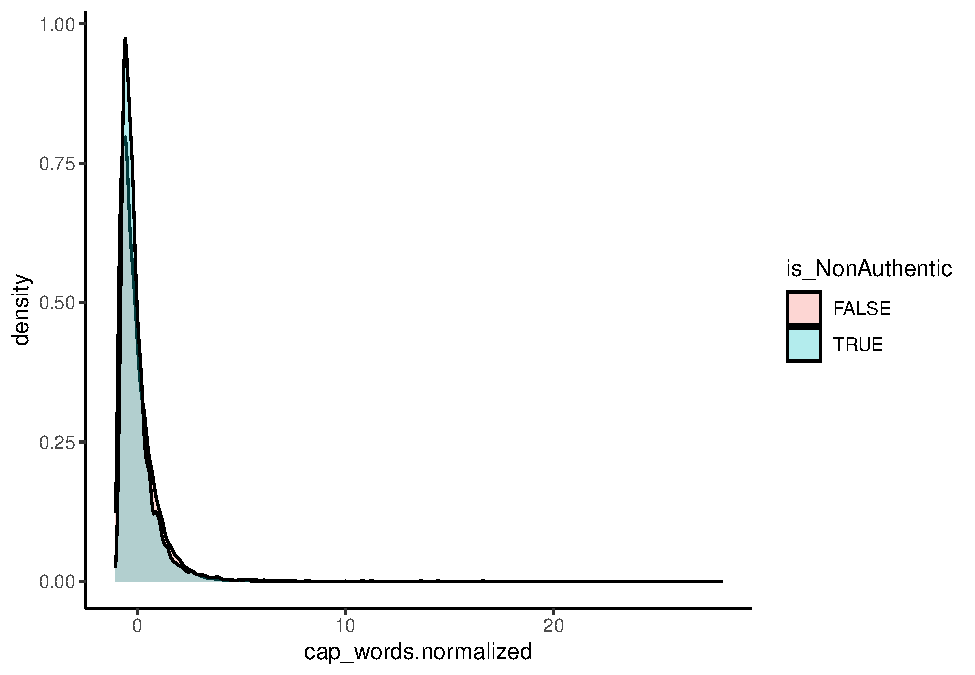
\includegraphics{report_files/figure-latex/visualize_capitalized_word_counts-1.pdf}

While their magnitudes may differ, their shapes are remarkably similar.
Using just the titles, we can perform the same analysis.

\begin{Shaded}
\begin{Highlighting}[]
\CommentTok{\# Count occurrences of whole words that are capitalized in just the title}
\NormalTok{all.news[, cap\_words }\SpecialCharTok{:}\ErrorTok{=} \FunctionTok{str\_count}\NormalTok{(title, }\StringTok{"[\^{}a{-}z][A{-}Z]+[\^{}a{-}z]"}\NormalTok{)]}

\CommentTok{\# normalize both sets of data separately, then plot}
\NormalTok{all.news[}
\NormalTok{  is\_NonAuthentic }\SpecialCharTok{==} \ConstantTok{TRUE}\NormalTok{,}
\NormalTok{  cap\_words.normalized }\SpecialCharTok{:}\ErrorTok{=}\NormalTok{ (cap\_words }\SpecialCharTok{{-}} \FunctionTok{mean}\NormalTok{(cap\_words))}\SpecialCharTok{/}\FunctionTok{sd}\NormalTok{(cap\_words)}
\NormalTok{][}
\NormalTok{  is\_NonAuthentic }\SpecialCharTok{==} \ConstantTok{FALSE}\NormalTok{,}
\NormalTok{  cap\_words.normalized }\SpecialCharTok{:}\ErrorTok{=}\NormalTok{ (cap\_words }\SpecialCharTok{{-}} \FunctionTok{mean}\NormalTok{(cap\_words))}\SpecialCharTok{/}\FunctionTok{sd}\NormalTok{(cap\_words)}
\NormalTok{]}

\CommentTok{\# plot}
\NormalTok{all.news }\SpecialCharTok{\%\textgreater{}\%}
  \FunctionTok{ggplot}\NormalTok{(}\FunctionTok{aes}\NormalTok{(}\AttributeTok{x =}\NormalTok{ cap\_words.normalized, }\AttributeTok{fill =}\NormalTok{ is\_NonAuthentic)) }\SpecialCharTok{+}
  \FunctionTok{geom\_density}\NormalTok{(}\AttributeTok{alpha =} \FloatTok{0.3}\NormalTok{)}
\end{Highlighting}
\end{Shaded}

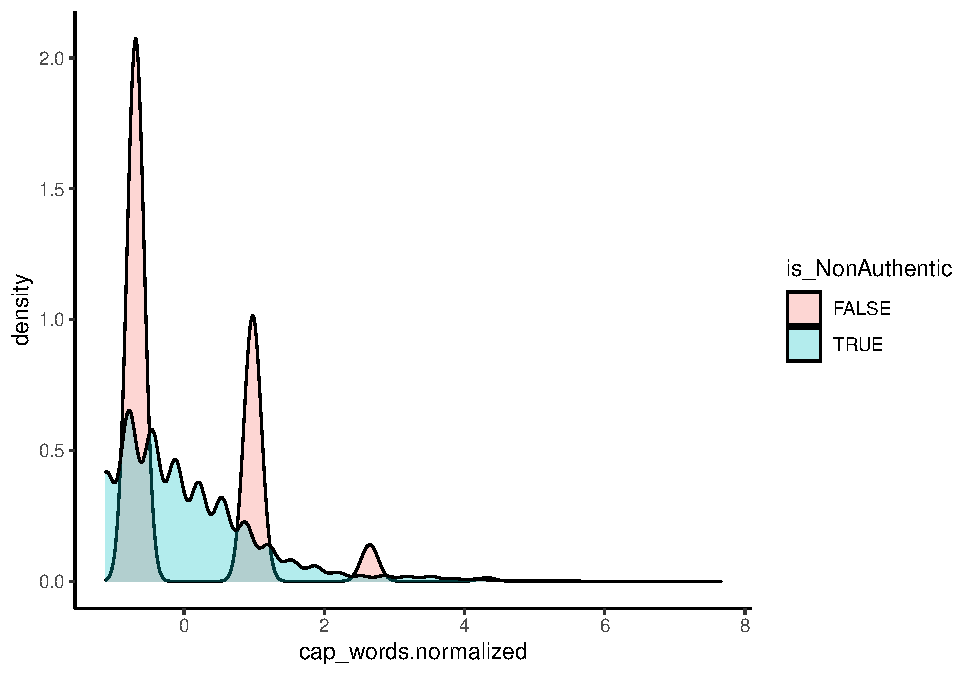
\includegraphics{report_files/figure-latex/visualize_capitalized_word_counts_just_title-1.pdf}

It is possible that titles have fewer words, so we end up with a lot of
divergent density plots. One of our predictors will be the number of
capitalized words in the title.

\pagebreak

Additionally, these data sources included a column of subjects. In
addition, it is clear that another bias is inherent in this study, in
that the subjects found in the Non-Authentic.csv data are absent from
the Authentic.csv data and vice versa.

\begin{Shaded}
\begin{Highlighting}[]
\CommentTok{\# Viewing all Subjects}
\NormalTok{all.news[, .N, by }\OtherTok{=}\NormalTok{ subject]}
\end{Highlighting}
\end{Shaded}

\begin{verbatim}
##            subject     N
## 1:    politicsNews 11272
## 2:       worldnews 10144
## 3:            News  9049
## 4:        politics  6837
## 5: Government News  1569
## 6:       left-news  4457
## 7:         US_News   783
## 8:     Middle-east   778
\end{verbatim}

\begin{Shaded}
\begin{Highlighting}[]
\CommentTok{\# Viewing subjects disaggregated by is\_NonAuthentic}
\NormalTok{all.news[, .N, by }\OtherTok{=} \FunctionTok{list}\NormalTok{(subject, is\_NonAuthentic)]}
\end{Highlighting}
\end{Shaded}

\begin{verbatim}
##            subject is_NonAuthentic     N
## 1:    politicsNews           FALSE 11272
## 2:       worldnews           FALSE 10144
## 3:            News            TRUE  9049
## 4:        politics            TRUE  6837
## 5: Government News            TRUE  1569
## 6:       left-news            TRUE  4457
## 7:         US_News            TRUE   783
## 8:     Middle-east            TRUE   778
\end{verbatim}

The observations are also all dated in some way. Although the vast
majority of dates here are from 2016-2018, the spread is not uniform.
Several dates fail to parse when this step is run. The inspection of
these failures (not shown here) reveals that 35 observations use a
different date format, and ten observations have URLs in the date
column. This data needs to be consistently imputed if we wish to use it
later. The URLs contain dates, which could be corrected by hand, but
after this point in analysis, the date column is not leveraged.

\pagebreak

\begin{Shaded}
\begin{Highlighting}[]
\CommentTok{\# Parse the date in an R date object}
\NormalTok{all.news[, parsed\_date }\SpecialCharTok{:}\ErrorTok{=} \FunctionTok{mdy}\NormalTok{(date)]}

\CommentTok{\# plot counts over time}
\NormalTok{all.news[, .N, by }\OtherTok{=}\NormalTok{ .(is\_NonAuthentic, }\AttributeTok{date =} \FunctionTok{date}\NormalTok{(parsed\_date))] }\SpecialCharTok{\%\textgreater{}\%}
  \FunctionTok{ggplot}\NormalTok{(}\FunctionTok{aes}\NormalTok{(}\AttributeTok{x =}\NormalTok{ date, }\AttributeTok{y =}\NormalTok{ N, }\AttributeTok{fill =}\NormalTok{ is\_NonAuthentic)) }\SpecialCharTok{+}
  \FunctionTok{stat\_smooth}\NormalTok{(}
    \AttributeTok{geom =} \StringTok{\textquotesingle{}area\textquotesingle{}}\NormalTok{,}
    \AttributeTok{span =} \FloatTok{0.25}\NormalTok{,}
    \AttributeTok{alpha =} \FloatTok{0.5}\NormalTok{,}
    \AttributeTok{method =} \StringTok{\textquotesingle{}loess\textquotesingle{}}\NormalTok{,}
    \AttributeTok{position =} \StringTok{"stack"}
\NormalTok{  )}
\end{Highlighting}
\end{Shaded}

\begin{verbatim}
## `geom_smooth()` using formula 'y ~ x'
\end{verbatim}

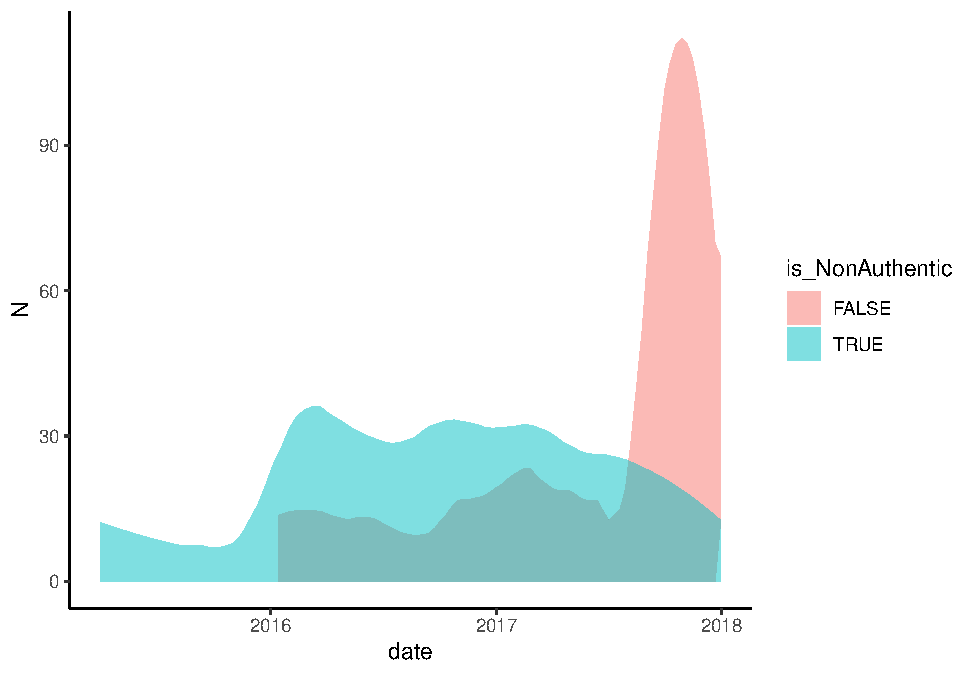
\includegraphics{report_files/figure-latex/parse_and_explore_dates-1.pdf}

\pagebreak

\hypertarget{approaches-and-models}{%
\subsection{Approaches and Models}\label{approaches-and-models}}

\hypertarget{data-preparation}{%
\paragraph{Data Preparation}\label{data-preparation}}

Our first step in the analysis will be to clean the data, tokenize the
texts, bind the tokens with the corresponding sentiments in each of the
three lexicons, and finally aggregate the resulting sentiments with
respect to each article.

Tokenization will take place per word for this dataset. Tokenization by
ngrams or n words is commonly used for in-depth analysis. These are
typically represented by bigrams, i.e.~pairs of words, allowing a
difference to be detected between tokens such as ``successful'' and
their inverse sentiment, ``not successful.''

Tokenized values also undergo another cleaning step: stopwords are
removed. There are several stop words, including ``and,'' ``is,'' and
``so.'' As such, they are no longer included in the analysis.

Additionally, it is important to note that merging tokens and sentiment
sets is performed using \emph{inner\_join}, which will inherently reduce
the size of the tokenized data list to only those rows in which there is
an appropriate sentiment. Because of this, lexicon size is a key factor
to consider when selecting one for analysis.

Additionally, we will divide the data into a training set and a test set
to ensure the accuracy of our models.

\begin{Shaded}
\begin{Highlighting}[]
\CommentTok{\# Clean and tidy dataset}
\NormalTok{all.news }\OtherTok{\textless{}{-}} \FunctionTok{lazy\_dt}\NormalTok{(all.news) }\SpecialCharTok{\%\textgreater{}\%}
  \FunctionTok{mutate}\NormalTok{(}
    \AttributeTok{title =} \FunctionTok{str\_trim}\NormalTok{(}\FunctionTok{iconv}\NormalTok{(title, }\AttributeTok{from =} \StringTok{"utf8"}\NormalTok{, }\AttributeTok{to =} \StringTok{"latin1"}\NormalTok{)),}
    \AttributeTok{text =} \FunctionTok{str\_trim}\NormalTok{(}\FunctionTok{iconv}\NormalTok{(text, }\AttributeTok{from =} \StringTok{"utf8"}\NormalTok{, }\AttributeTok{to =} \StringTok{"latin1"}\NormalTok{))}
\NormalTok{  ) }\SpecialCharTok{\%\textgreater{}\%}
  \FunctionTok{filter}\NormalTok{(}\SpecialCharTok{!}\FunctionTok{is.na}\NormalTok{(title) }\SpecialCharTok{\&}\NormalTok{ title }\SpecialCharTok{!=} \StringTok{\textquotesingle{}\textquotesingle{}}\NormalTok{) }\SpecialCharTok{\%\textgreater{}\%}
  \FunctionTok{mutate}\NormalTok{(}
    \AttributeTok{full\_text =} \FunctionTok{paste}\NormalTok{(text, title),}
    \AttributeTok{is\_NonAuthentic =} \FunctionTok{as.factor}\NormalTok{(is\_NonAuthentic),}
    \AttributeTok{title\_caps =} \FunctionTok{str\_count}\NormalTok{(title, }\StringTok{"[\^{}a{-}z][A{-}Z]+[\^{}a{-}z]"}\NormalTok{)}
\NormalTok{  ) }\SpecialCharTok{\%\textgreater{}\%}
  \FunctionTok{select}\NormalTok{(title, full\_text, is\_NonAuthentic, title\_caps) }\SpecialCharTok{\%\textgreater{}\%}
  \FunctionTok{as.data.table}\NormalTok{()}

\CommentTok{\# Mark training and test datasets.}
\NormalTok{train.index }\OtherTok{\textless{}{-}} \FunctionTok{createDataPartition}\NormalTok{(}
\NormalTok{  all.news}\SpecialCharTok{$}\NormalTok{is\_NonAuthentic,}
  \AttributeTok{p =} \FloatTok{0.8}\NormalTok{,}
  \AttributeTok{times =} \DecValTok{1}\NormalTok{,}
  \AttributeTok{list =} \ConstantTok{FALSE}
\NormalTok{)}

\NormalTok{all.news}\SpecialCharTok{$}\NormalTok{set }\OtherTok{\textless{}{-}} \StringTok{"testing"}
\NormalTok{all.news[train.index, set }\SpecialCharTok{:}\ErrorTok{=} \StringTok{"training"}\NormalTok{]}

\FunctionTok{remove}\NormalTok{(train.index)}

\CommentTok{\# split tokens for joining sentiment, remove stop words.}
\CommentTok{\# This takes a few moments}
\NormalTok{tokenized }\OtherTok{\textless{}{-}}\NormalTok{ all.news }\SpecialCharTok{\%\textgreater{}\%}
  \FunctionTok{unnest\_tokens}\NormalTok{(token, full\_text) }\SpecialCharTok{\%\textgreater{}\%}
  \FunctionTok{lazy\_dt}\NormalTok{() }\SpecialCharTok{\%\textgreater{}\%}
  \FunctionTok{anti\_join}\NormalTok{(}\FunctionTok{data.table}\NormalTok{(}\AttributeTok{token =}\NormalTok{ stop\_words}\SpecialCharTok{$}\NormalTok{word), }\AttributeTok{by =} \StringTok{"token"}\NormalTok{) }\SpecialCharTok{\%\textgreater{}\%}
  \FunctionTok{as.data.table}\NormalTok{()}
\end{Highlighting}
\end{Shaded}

Each of the three lexicons will now be attached to these tokens
separately. Each lexicon provides a different measure of sentiment, so
different aggregations will be required. Affin lexicon provides an
integer column with a simple summation method.

\begin{Shaded}
\begin{Highlighting}[]
\CommentTok{\# Read the data from file}
\NormalTok{afinn }\OtherTok{\textless{}{-}} \FunctionTok{fread}\NormalTok{(}\StringTok{"./data/afinn.csv"}\NormalTok{)}

\CommentTok{\# Change names of columns for joining}
\FunctionTok{setnames}\NormalTok{(afinn, }\FunctionTok{c}\NormalTok{(}\StringTok{"token"}\NormalTok{, }\StringTok{"sentiment"}\NormalTok{))}

\CommentTok{\# setting data.table keys make joins a lot faster}
\FunctionTok{setkey}\NormalTok{(afinn, token)}
\FunctionTok{setkey}\NormalTok{(tokenized, token)}

\CommentTok{\# data.table syntax for doing an inner join on keyed data.tables}
\NormalTok{afinn }\OtherTok{\textless{}{-}}\NormalTok{ afinn[tokenized, nomatch }\OtherTok{=} \ConstantTok{NULL}\NormalTok{]}

\CommentTok{\# aggregate total sentiment for each article}
\NormalTok{afinn }\OtherTok{\textless{}{-}}\NormalTok{ afinn[}
\NormalTok{  ,}
  \FunctionTok{list}\NormalTok{(}\AttributeTok{sentiment =} \FunctionTok{sum}\NormalTok{(sentiment)),}
\NormalTok{  by  }\OtherTok{=} \FunctionTok{list}\NormalTok{(title, is\_NonAuthentic, title\_caps, set)}
\NormalTok{]}
\end{Highlighting}
\end{Shaded}

To aggregate the NRC lexicon requires far more effort. Our first step is
to join the tokens to the dataset, which eliminates all words that are
not present in the NRC lexicon. However, this same join also multiplies
many of the rows by the number of sentiments a token has. To aggregate
these multiple rows into columns, we must first create an intermediary
process that shows whether or not a given token has the attached
sentiments. Afterwards, these can be aggregated into per-article totals.

\begin{Shaded}
\begin{Highlighting}[]
\NormalTok{nrc }\OtherTok{\textless{}{-}} \FunctionTok{fread}\NormalTok{(}\StringTok{"./data/nrc.csv"}\NormalTok{)}

\CommentTok{\# Change column names for joining}
\FunctionTok{setnames}\NormalTok{(nrc, }\StringTok{"word"}\NormalTok{, }\StringTok{"token"}\NormalTok{)}

\CommentTok{\# Set keys for data.table join}
\FunctionTok{setkey}\NormalTok{(nrc, token)}
\FunctionTok{setkey}\NormalTok{(tokenized, token)}

\CommentTok{\# data.table syntax for doing an inner join on keyed data.tables}
\NormalTok{nrc }\OtherTok{\textless{}{-}}\NormalTok{ nrc[tokenized, nomatch }\OtherTok{=} \ConstantTok{NULL}\NormalTok{]}

\CommentTok{\# Tibbles with pivot\_wider is a much easier{-}to{-}read approach here,}
\CommentTok{\# but there are other more performant ways of doing this if our}
\CommentTok{\# dataset was very large. See \textasciigrave{}reshape2\textasciigrave{} package}
\NormalTok{nrc }\OtherTok{\textless{}{-}} \FunctionTok{as\_tibble}\NormalTok{(nrc) }\SpecialCharTok{\%\textgreater{}\%}
  \FunctionTok{pivot\_wider}\NormalTok{(}
    \AttributeTok{names\_from =}\NormalTok{ sentiment,}
    \AttributeTok{values\_from =}\NormalTok{ sentiment,}
    \AttributeTok{values\_fn =} \FunctionTok{list}\NormalTok{(}\AttributeTok{sentiment =}\NormalTok{ length),}
    \AttributeTok{values\_fill =} \FunctionTok{list}\NormalTok{(}\AttributeTok{sentiment =} \DecValTok{0}\NormalTok{)}
\NormalTok{  )}

\CommentTok{\# View the wide output of this table}
\FunctionTok{head}\NormalTok{(nrc, }\DecValTok{3}\NormalTok{)}
\end{Highlighting}
\end{Shaded}

\begin{verbatim}
## # A tibble: 3 x 15
##   token  title     is_NonAuthentic title_caps set   trust  fear negative sadness
##   <chr>  <chr>     <fct>                <int> <chr> <int> <int>    <int>   <int>
## 1 abacus Canada's~ FALSE                    0 trai~     1     0        0       0
## 2 aband~ Spy chie~ FALSE                    0 test~     0     1        1       1
## 3 aband~ Schumer:~ FALSE                    0 trai~     0     1        1       1
## # ... with 6 more variables: anger <int>, surprise <int>, positive <int>,
## #   disgust <int>, anticipation <int>, joy <int>
\end{verbatim}

\begin{Shaded}
\begin{Highlighting}[]
\CommentTok{\# Roll up counts of all sentiments for all tokens for each article, ie Anger: 5, Joy 0, Negative: 3}
\NormalTok{nrc }\OtherTok{\textless{}{-}}\NormalTok{ nrc }\SpecialCharTok{\%\textgreater{}\%}
  \FunctionTok{group\_by}\NormalTok{(title, is\_NonAuthentic, title\_caps, set) }\SpecialCharTok{\%\textgreater{}\%}
  \FunctionTok{summarize\_at}\NormalTok{(}\FunctionTok{vars}\NormalTok{(}\SpecialCharTok{{-}}\NormalTok{token), }\FunctionTok{list}\NormalTok{(sum)) }\SpecialCharTok{\%\textgreater{}\%}
  \FunctionTok{as.data.table}\NormalTok{()}

\FunctionTok{head}\NormalTok{(nrc, }\DecValTok{3}\NormalTok{)}
\end{Highlighting}
\end{Shaded}

\begin{verbatim}
##                                                                          title
## 1:     '#1 In Bigotry': Twitter EVISCERATES Mississippi Gov. Over Anti-Gay Law
## 2: '60 MINUTES': 9/11 REPORT Could Incriminate Saudi Arabia With These Details
## 3:          'A better future' - Britain's May tries to rally her Conservatives
##    is_NonAuthentic title_caps      set trust fear negative sadness anger
## 1:            TRUE          1 training    21   15       17      13    14
## 2:            TRUE          2 training    12    9       10       6     6
## 3:           FALSE          1 training    23   10       20      10    11
##    surprise positive disgust anticipation joy
## 1:        2       18      11           10   7
## 2:        3       16       1           10   6
## 3:        4       38       5           10  11
\end{verbatim}

As a final note, the NRC VAD lexicon has been aggregated like Afinn's,
but with columns for each dimension.

\begin{Shaded}
\begin{Highlighting}[]
\CommentTok{\# Read the NRC VAD data from file}
\NormalTok{vad }\OtherTok{\textless{}{-}} \FunctionTok{fread}\NormalTok{(}\StringTok{"./data/nrc\_vad.csv"}\NormalTok{)}

\CommentTok{\# This lexicon comes with Title{-}cased columns}
\FunctionTok{setnames}\NormalTok{(vad, }\FunctionTok{tolower}\NormalTok{(}\FunctionTok{names}\NormalTok{(vad)))}

\CommentTok{\# change this column name for joining}
\FunctionTok{setnames}\NormalTok{(vad, }\StringTok{"word"}\NormalTok{, }\StringTok{"token"}\NormalTok{)}

\FunctionTok{setkey}\NormalTok{(vad, token)}
\FunctionTok{setkey}\NormalTok{(tokenized, token)}

\CommentTok{\# data.table syntax for an inner join on keyed data.tables}
\NormalTok{vad }\OtherTok{\textless{}{-}}\NormalTok{ vad[tokenized, nomatch }\OtherTok{=} \ConstantTok{NULL}\NormalTok{]}

\CommentTok{\# Aggregate dimensions by summing across articles}
\NormalTok{vad }\OtherTok{\textless{}{-}}\NormalTok{ vad[}
\NormalTok{  ,}
  \FunctionTok{list}\NormalTok{(}
    \AttributeTok{valence =} \FunctionTok{sum}\NormalTok{(valence),}
    \AttributeTok{arousal =} \FunctionTok{sum}\NormalTok{(arousal),}
    \AttributeTok{dominance =} \FunctionTok{sum}\NormalTok{(dominance)}
\NormalTok{  ),}
\NormalTok{  by }\OtherTok{=} \FunctionTok{list}\NormalTok{(title, is\_NonAuthentic, title\_caps, set)}
\NormalTok{]}
\end{Highlighting}
\end{Shaded}

The test and training sets can now be separated. The data sets were kept
together for processing because the above data preparation relies
heavily on merges. The training and testing identifiers will be
separated here.

\begin{Shaded}
\begin{Highlighting}[]
\NormalTok{afinn }\OtherTok{\textless{}{-}} \FunctionTok{split}\NormalTok{(afinn, }\AttributeTok{by =} \StringTok{"set"}\NormalTok{, }\AttributeTok{keep.by =} \ConstantTok{FALSE}\NormalTok{)}
\NormalTok{afinn.training }\OtherTok{\textless{}{-}}\NormalTok{ afinn}\SpecialCharTok{$}\NormalTok{training}
\NormalTok{afinn.testing }\OtherTok{\textless{}{-}}\NormalTok{ afinn}\SpecialCharTok{$}\NormalTok{testing}

\NormalTok{nrc }\OtherTok{\textless{}{-}} \FunctionTok{split}\NormalTok{(nrc, }\AttributeTok{by =} \StringTok{"set"}\NormalTok{, }\AttributeTok{keep.by =} \ConstantTok{FALSE}\NormalTok{)}
\NormalTok{nrc.training }\OtherTok{\textless{}{-}}\NormalTok{ nrc}\SpecialCharTok{$}\NormalTok{training}
\NormalTok{nrc.testing }\OtherTok{\textless{}{-}}\NormalTok{ nrc}\SpecialCharTok{$}\NormalTok{testing}

\NormalTok{vad }\OtherTok{\textless{}{-}} \FunctionTok{split}\NormalTok{(vad, }\AttributeTok{by =} \StringTok{"set"}\NormalTok{, }\AttributeTok{keep.by =} \ConstantTok{FALSE}\NormalTok{)}
\NormalTok{vad.training }\OtherTok{\textless{}{-}}\NormalTok{ vad}\SpecialCharTok{$}\NormalTok{training}
\NormalTok{vad.testing }\OtherTok{\textless{}{-}}\NormalTok{ vad}\SpecialCharTok{$}\NormalTok{testing}

\CommentTok{\# clean up unneded objects}
\FunctionTok{remove}\NormalTok{(tokenized, afinn, nrc, vad)}
\end{Highlighting}
\end{Shaded}

\hypertarget{naive-baseline}{%
\paragraph{Naive Baseline}\label{naive-baseline}}

Using the most naive approach as a baseline always proves to be
instructive. The intended inference can be summed up by tossing a coin
and guessing accordingly. We can predict that based on the observed
data, this would be approximately half the time correct given a normal
distribution of binary categorical outcomes. Exactly 50\% of the time,
this holds true for the observed data.

\begin{Shaded}
\begin{Highlighting}[]
\CommentTok{\# Replicate the naive approach 10000 times}
\FunctionTok{mean}\NormalTok{(}\FunctionTok{replicate}\NormalTok{(}\DecValTok{10000}\NormalTok{, \{}
  \CommentTok{\# Guess True or False for is\_NonAuthentic randomly}
\NormalTok{  predictions }\OtherTok{\textless{}{-}} \FunctionTok{sample}\NormalTok{(}\FunctionTok{c}\NormalTok{(}\ConstantTok{TRUE}\NormalTok{, }\ConstantTok{FALSE}\NormalTok{), }\FunctionTok{nrow}\NormalTok{(all.news), }\AttributeTok{replace =} \ConstantTok{TRUE}\NormalTok{)}
  
  \CommentTok{\# Return the accuracy of this replication}
  \FunctionTok{mean}\NormalTok{(predictions }\SpecialCharTok{==}\NormalTok{ all.news}\SpecialCharTok{$}\NormalTok{is\_NonAuthentic)}
\NormalTok{\}))}
\end{Highlighting}
\end{Shaded}

\begin{verbatim}
## [1] 0.5
\end{verbatim}

\hypertarget{random-forests}{%
\paragraph{Random Forests}\label{random-forests}}

Due to the numerical and continuous nature of our predictors, decision
trees are a very common classification algorithm. Each set of data will
be mapped to a sentiment lexicon by creating and training a model. Using
\emph{parRF}, a parallelized Random Forest implementation, this analysis
is accomplished more quickly. This package's caret training method only
has one tuning parameter, \emph{mtry}, and I've been satisfied with the
default settings for small data sets. I have implemented this here on a
consumer PC with a roughly 4Ghz processor running 16 threads.

\begin{Shaded}
\begin{Highlighting}[]
\CommentTok{\# We can leveraging matrix{-}based function signatures for all the models we build}
\CommentTok{\# This helper function will create a matrix of all predictors from a given data.table}
\NormalTok{makePredictors }\OtherTok{\textless{}{-}} \ControlFlowTok{function}\NormalTok{(dt) \{}
  \CommentTok{\# drop our title, used only as an identifier column}
\NormalTok{  dt}\SpecialCharTok{$}\NormalTok{title }\OtherTok{=} \ConstantTok{NULL}

  \CommentTok{\# drop the response column}
\NormalTok{  dt}\SpecialCharTok{$}\NormalTok{is\_NonAuthentic }\OtherTok{=} \ConstantTok{NULL}

  \CommentTok{\# return the rest of the columns as a matrix}
  \FunctionTok{as.matrix}\NormalTok{(dt)}
\NormalTok{\}}

\CommentTok{\# Start and register parallel threads}
\CommentTok{\# NB: Never set this number higher than your computer}
\CommentTok{\# can handle!   }
\NormalTok{nThreads }\OtherTok{\textless{}{-}} \DecValTok{16}
\NormalTok{cl }\OtherTok{\textless{}{-}} \FunctionTok{makeSOCKcluster}\NormalTok{(nThreads)}
\FunctionTok{registerDoSNOW}\NormalTok{(cl)}

\CommentTok{\# A \textasciigrave{}caret\textasciigrave{} trainControl object, using parallized}
\CommentTok{\# 5{-}fold cross{-}validation.}
\NormalTok{rf.trainControl }\OtherTok{\textless{}{-}} \FunctionTok{trainControl}\NormalTok{(}
  \AttributeTok{method =} \StringTok{"cv"}\NormalTok{,}
  \AttributeTok{number =} \DecValTok{5}\NormalTok{,}
  \AttributeTok{allowParallel =} \ConstantTok{TRUE}
\NormalTok{)}

\CommentTok{\# RF model for Afinn sentiments}
\NormalTok{afinn.rf.model }\OtherTok{\textless{}{-}} \FunctionTok{train}\NormalTok{(}
  \FunctionTok{makePredictors}\NormalTok{(afinn.training),}
\NormalTok{  afinn.training}\SpecialCharTok{$}\NormalTok{is\_NonAuthentic,}
  \AttributeTok{method =} \StringTok{"parRF"}\NormalTok{,}
  \AttributeTok{trControl =}\NormalTok{ rf.trainControl}
\NormalTok{)}
\end{Highlighting}
\end{Shaded}

\begin{verbatim}
## note: only 1 unique complexity parameters in default grid. Truncating the grid to 1 .
\end{verbatim}

\begin{Shaded}
\begin{Highlighting}[]
\CommentTok{\# RF NRC}
\NormalTok{nrc.rf.model }\OtherTok{\textless{}{-}} \FunctionTok{train}\NormalTok{(}
  \FunctionTok{makePredictors}\NormalTok{(nrc.training),}
\NormalTok{  nrc.training}\SpecialCharTok{$}\NormalTok{is\_NonAuthentic,}
  \AttributeTok{method =} \StringTok{"parRF"}\NormalTok{,}
  \AttributeTok{trControl =}\NormalTok{ rf.trainControl}
\NormalTok{)}

\CommentTok{\# RF VAD}
\NormalTok{vad.rf.model }\OtherTok{\textless{}{-}} \FunctionTok{train}\NormalTok{(}
  \FunctionTok{makePredictors}\NormalTok{(vad.training),}
\NormalTok{  vad.training}\SpecialCharTok{$}\NormalTok{is\_NonAuthentic,}
  \AttributeTok{method =} \StringTok{"parRF"}\NormalTok{,}
  \AttributeTok{trControl =}\NormalTok{ rf.trainControl}
\NormalTok{)}

\CommentTok{\# Stop and de{-}register parallel computing}
\FunctionTok{stopCluster}\NormalTok{(cl)}
\FunctionTok{registerDoSEQ}\NormalTok{()}
\FunctionTok{remove}\NormalTok{(cl)}
\end{Highlighting}
\end{Shaded}

We can now evaluate the models' accuracy by comparing them to the
training data with which they were built. While this is obviously
overfit, it does begin to show us if these attempts were even close to
succeeding.

\begin{Shaded}
\begin{Highlighting}[]
\DocumentationTok{\#\# Accuracy measures against training datasets}
\CommentTok{\# Afinn RF}
\FunctionTok{confusionMatrix}\NormalTok{(}\FunctionTok{fitted}\NormalTok{(afinn.rf.model), afinn.training}\SpecialCharTok{$}\NormalTok{is\_NonAuthentic)}
\end{Highlighting}
\end{Shaded}

\begin{verbatim}
## Confusion Matrix and Statistics
## 
##           Reference
## Prediction FALSE  TRUE
##      FALSE 14847  4057
##      TRUE   1523 10859
##                                         
##                Accuracy : 0.822         
##                  95% CI : (0.817, 0.826)
##     No Information Rate : 0.523         
##     P-Value [Acc > NIR] : <2e-16        
##                                         
##                   Kappa : 0.64          
##                                         
##  Mcnemar's Test P-Value : <2e-16        
##                                         
##             Sensitivity : 0.907         
##             Specificity : 0.728         
##          Pos Pred Value : 0.785         
##          Neg Pred Value : 0.877         
##              Prevalence : 0.523         
##          Detection Rate : 0.475         
##    Detection Prevalence : 0.604         
##       Balanced Accuracy : 0.817         
##                                         
##        'Positive' Class : FALSE         
## 
\end{verbatim}

\begin{Shaded}
\begin{Highlighting}[]
\CommentTok{\# 82.2\%}

\CommentTok{\# NRC RF}
\FunctionTok{confusionMatrix}\NormalTok{(}\FunctionTok{fitted}\NormalTok{(nrc.rf.model), nrc.training}\SpecialCharTok{$}\NormalTok{is\_NonAuthentic)}
\end{Highlighting}
\end{Shaded}

\begin{verbatim}
## Confusion Matrix and Statistics
## 
##           Reference
## Prediction FALSE  TRUE
##      FALSE 16724    81
##      TRUE     12 15039
##                                         
##                Accuracy : 0.997         
##                  95% CI : (0.996, 0.998)
##     No Information Rate : 0.525         
##     P-Value [Acc > NIR] : < 2e-16       
##                                         
##                   Kappa : 0.994         
##                                         
##  Mcnemar's Test P-Value : 1.77e-12      
##                                         
##             Sensitivity : 0.999         
##             Specificity : 0.995         
##          Pos Pred Value : 0.995         
##          Neg Pred Value : 0.999         
##              Prevalence : 0.525         
##          Detection Rate : 0.525         
##    Detection Prevalence : 0.528         
##       Balanced Accuracy : 0.997         
##                                         
##        'Positive' Class : FALSE         
## 
\end{verbatim}

\begin{Shaded}
\begin{Highlighting}[]
\CommentTok{\# 99.7\%}

\CommentTok{\# NRC VAD RF}
\FunctionTok{confusionMatrix}\NormalTok{(}\FunctionTok{fitted}\NormalTok{(vad.rf.model), vad.training}\SpecialCharTok{$}\NormalTok{is\_NonAuthentic)}
\end{Highlighting}
\end{Shaded}

\begin{verbatim}
## Confusion Matrix and Statistics
## 
##           Reference
## Prediction FALSE  TRUE
##      FALSE 16726    35
##      TRUE     17 15133
##                                         
##                Accuracy : 0.998         
##                  95% CI : (0.998, 0.999)
##     No Information Rate : 0.525         
##     P-Value [Acc > NIR] : <2e-16        
##                                         
##                   Kappa : 0.997         
##                                         
##  Mcnemar's Test P-Value : 0.0184        
##                                         
##             Sensitivity : 0.999         
##             Specificity : 0.998         
##          Pos Pred Value : 0.998         
##          Neg Pred Value : 0.999         
##              Prevalence : 0.525         
##          Detection Rate : 0.524         
##    Detection Prevalence : 0.525         
##       Balanced Accuracy : 0.998         
##                                         
##        'Positive' Class : FALSE         
## 
\end{verbatim}

\begin{Shaded}
\begin{Highlighting}[]
\CommentTok{\# 99.8\%}
\end{Highlighting}
\end{Shaded}

\hypertarget{support-vector-machines}{%
\paragraph{Support Vector Machines}\label{support-vector-machines}}

Support Vector Machines are mathematically based models that draw
boundaries around collections of data in higher-order planes. It is
important to note that the \emph{ksvm} function used here, as well as
the analysis at large, is a type of SVM that leverages something called
the \emph{kernel trick}: an ingenious application of mathematical
assumptions that makes SVMs work well in higher dimensions. TIt is not
my purpose to describe the mathematics of SVMs in this paper, so I will
demonstrate their ability to separate clusters of data visually.

\begin{Shaded}
\begin{Highlighting}[]
\CommentTok{\# Grab a very small chunk of data to demonstrate with}
\CommentTok{\# 500 rows, with only "joy" and "disgust" dimensions as predictors}
\NormalTok{data.small }\OtherTok{\textless{}{-}}\NormalTok{ nrc.training[}
  \FunctionTok{sample.int}\NormalTok{(}\FunctionTok{nrow}\NormalTok{(nrc.training), }\DecValTok{500}\NormalTok{),}
  \FunctionTok{list}\NormalTok{(is\_NonAuthentic, joy, disgust)}
\NormalTok{]}

\CommentTok{\# Scatterplot of the predictors, color coded by outcome}
\NormalTok{data.small }\SpecialCharTok{\%\textgreater{}\%}
  \FunctionTok{ggplot}\NormalTok{(}\FunctionTok{aes}\NormalTok{(}\AttributeTok{x =}\NormalTok{ joy, }\AttributeTok{y =}\NormalTok{ disgust, }\AttributeTok{color =}\NormalTok{ is\_NonAuthentic)) }\SpecialCharTok{+}
  \FunctionTok{geom\_point}\NormalTok{()}
\end{Highlighting}
\end{Shaded}

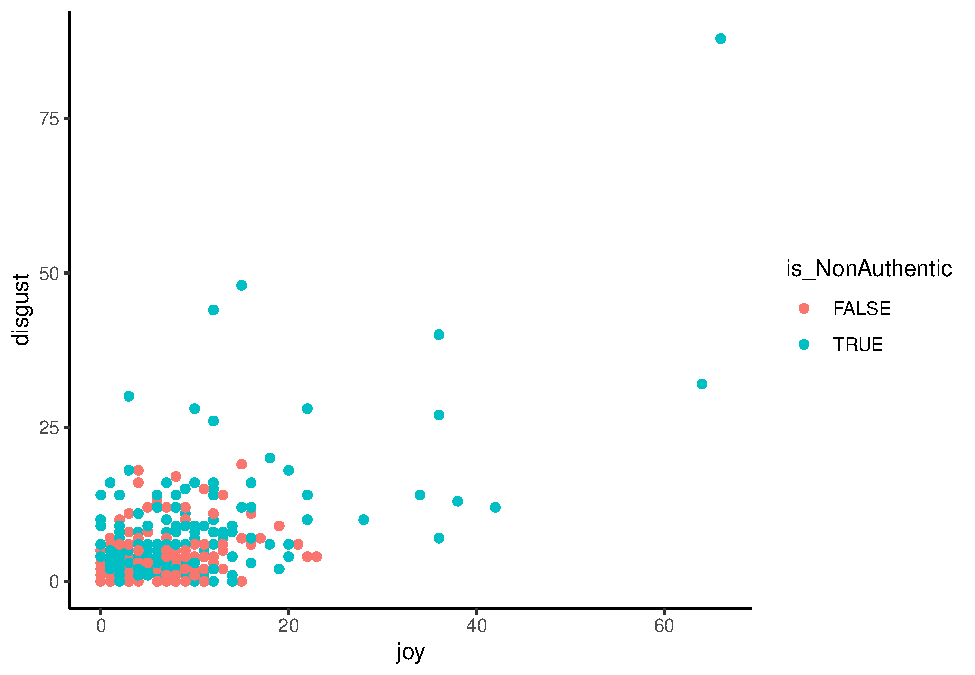
\includegraphics{report_files/figure-latex/illustrate_svm_prep-1.pdf}

As we can see, there does seem to be a general visual trend that one
color is more prevalent in the upper-right of the plot, while the
cluster in the lower left seems to be more focused on the other color.
Now we can train a model on this data.

\begin{Shaded}
\begin{Highlighting}[]
\CommentTok{\# Grab a matrix of predictors and a response vector}
\NormalTok{predictors }\OtherTok{\textless{}{-}} \FunctionTok{as.matrix}\NormalTok{(data.small[, .(joy, disgust)])}
\NormalTok{response }\OtherTok{\textless{}{-}}\NormalTok{ data.small}\SpecialCharTok{$}\NormalTok{is\_NonAuthentic}

\CommentTok{\# Train a basic KSVM model}
\NormalTok{ksvm.model }\OtherTok{\textless{}{-}} \FunctionTok{ksvm}\NormalTok{(}
  \AttributeTok{x =}\NormalTok{ predictors,}
  \AttributeTok{y =}\NormalTok{ response}
\NormalTok{)}

\CommentTok{\# Make predictions and view accuracy}
\NormalTok{ksvm.predictions }\OtherTok{\textless{}{-}} \FunctionTok{predict}\NormalTok{(}
\NormalTok{  ksvm.model,}
  \FunctionTok{as.matrix}\NormalTok{(nrc.training[, .(joy, disgust)])}
\NormalTok{)}
\FunctionTok{confusionMatrix}\NormalTok{(ksvm.predictions, nrc.training}\SpecialCharTok{$}\NormalTok{is\_NonAuthentic)}
\end{Highlighting}
\end{Shaded}

\begin{verbatim}
## Confusion Matrix and Statistics
## 
##           Reference
## Prediction FALSE  TRUE
##      FALSE 12219  7480
##      TRUE   4517  7640
##                                         
##                Accuracy : 0.623         
##                  95% CI : (0.618, 0.629)
##     No Information Rate : 0.525         
##     P-Value [Acc > NIR] : <2e-16        
##                                         
##                   Kappa : 0.238         
##                                         
##  Mcnemar's Test P-Value : <2e-16        
##                                         
##             Sensitivity : 0.730         
##             Specificity : 0.505         
##          Pos Pred Value : 0.620         
##          Neg Pred Value : 0.628         
##              Prevalence : 0.525         
##          Detection Rate : 0.384         
##    Detection Prevalence : 0.618         
##       Balanced Accuracy : 0.618         
##                                         
##        'Positive' Class : FALSE         
## 
\end{verbatim}

\begin{Shaded}
\begin{Highlighting}[]
\CommentTok{\# 62.3\%}
\end{Highlighting}
\end{Shaded}

The model's accuracy isn't surprising given the limited data and only
two dimensions. A similar scatterplot can be used to demonstrate the
boundaries of the model.

\begin{Shaded}
\begin{Highlighting}[]
\CommentTok{\# Visualize the Boundaries our KSVM model has created.}
\FunctionTok{plot}\NormalTok{(ksvm.model, }\AttributeTok{data =}\NormalTok{ predictors)}
\end{Highlighting}
\end{Shaded}

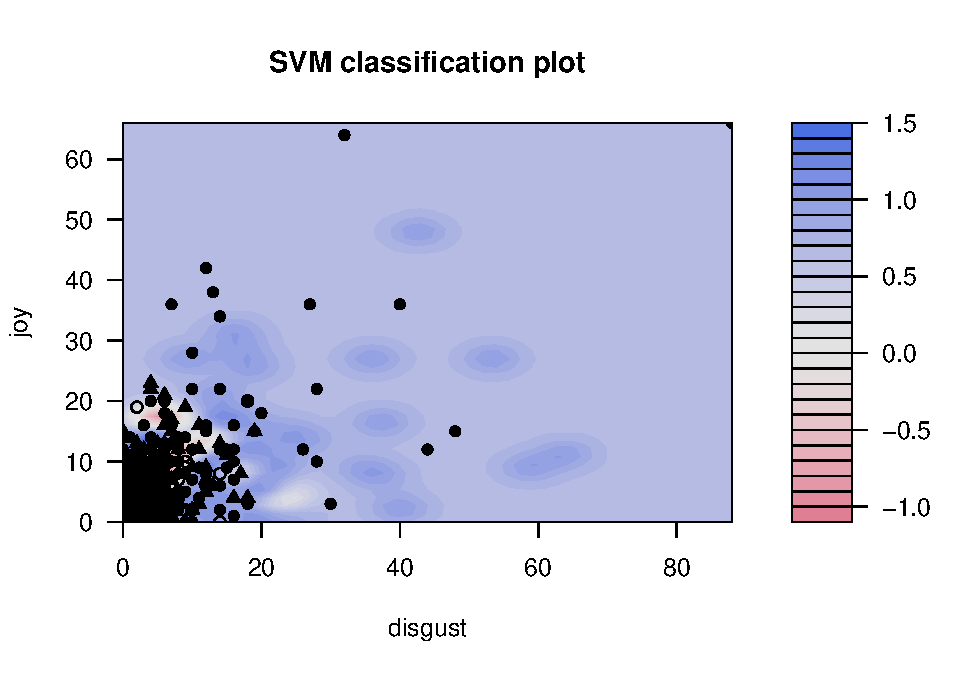
\includegraphics{report_files/figure-latex/illustrate_svm_boudaries-1.pdf}

It is clear that the model has a lot of learning to do, but the
boundaries drawn seem reasonable. Machine learning problems are often
complicated in the middle, so more data, more dimensions, and a better
algorithm should improve our results.

Our KSVM models are now ready for training. It is simply a matter of
training sigma, which affects how linear or flexible the decision
boundary becomes. In addition to \emph{C}, there is a cost parameter
that is used to penalize residuals that are too large after
normalization. I have left this as the default value of 1 due to the
relatively small size of our data.

As a result of a feature in the KernLab package named \emph{sigest}, the
tuning values for \emph{sigma} are estimated based on the data fractions
of the training set. This range has been expanded by 25 percent on
either side, covering a very large number of possible parameters. Each
model is trained using lexicon-bound training data, so this step is done
for every model.

\begin{Shaded}
\begin{Highlighting}[]
\CommentTok{\# Create and register threads for parallel computing}
\NormalTok{cl }\OtherTok{\textless{}{-}} \FunctionTok{makeSOCKcluster}\NormalTok{(nThreads)}
\FunctionTok{registerDoSNOW}\NormalTok{(cl)}

\CommentTok{\# Create a trainControl object for all KSVM models}
\NormalTok{ksvm.trainControl }\OtherTok{\textless{}{-}} \FunctionTok{trainControl}\NormalTok{(}
  \AttributeTok{method =} \StringTok{"cv"}\NormalTok{,}
  \AttributeTok{number =} \DecValTok{5}\NormalTok{,}
  \AttributeTok{allowParallel =} \ConstantTok{TRUE}
\NormalTok{)}

\CommentTok{\# Create the matrix of predictors}
\NormalTok{afinn.training.predictors }\OtherTok{\textless{}{-}} \FunctionTok{makePredictors}\NormalTok{(afinn.training)}

\CommentTok{\# Here, and below, sigmas are going to come from an estimation function provided}
\CommentTok{\# in the \textasciigrave{}kernlab\textasciigrave{} package. The range of these will be expanded by 25\% so that}
\CommentTok{\# we can try a broader set of values for sigma.}
\NormalTok{afinn.training.sigmas }\OtherTok{\textless{}{-}} \FunctionTok{sigest}\NormalTok{(afinn.training.predictors, }\AttributeTok{frac =} \DecValTok{1}\NormalTok{)}
\NormalTok{afinn.training.sigmas }\OtherTok{\textless{}{-}} \FunctionTok{seq}\NormalTok{(}
\NormalTok{  afinn.training.sigmas[}\StringTok{"90\%"}\NormalTok{] }\SpecialCharTok{*} \FloatTok{0.75}\NormalTok{,}
\NormalTok{  afinn.training.sigmas[}\StringTok{"10\%"}\NormalTok{] }\SpecialCharTok{*} \FloatTok{1.25}\NormalTok{,}
  \AttributeTok{length.out =} \DecValTok{10}
\NormalTok{)}

\CommentTok{\# train the model}
\NormalTok{afinn.ksvm.model }\OtherTok{\textless{}{-}} \FunctionTok{train}\NormalTok{(}
\NormalTok{  afinn.training.predictors,}
\NormalTok{  afinn.training}\SpecialCharTok{$}\NormalTok{is\_NonAuthentic,}
  \AttributeTok{method =} \StringTok{\textquotesingle{}svmRadial\textquotesingle{}}\NormalTok{,}
  \AttributeTok{trControl =}\NormalTok{ ksvm.trainControl,}
  \AttributeTok{tuneGrid =} \FunctionTok{data.table}\NormalTok{(}
    \AttributeTok{sigma =}\NormalTok{ afinn.training.sigmas,}
    \AttributeTok{C =} \DecValTok{1}
\NormalTok{  )}
\NormalTok{)}
\end{Highlighting}
\end{Shaded}

\begin{verbatim}
## Warning in (function (kind = NULL, normal.kind = NULL, sample.kind = NULL) :
## non-uniform 'Rounding' sampler used
\end{verbatim}

\begin{Shaded}
\begin{Highlighting}[]
\CommentTok{\# Create the matrix of predictors}
\NormalTok{nrc.training.predictors }\OtherTok{\textless{}{-}} \FunctionTok{makePredictors}\NormalTok{(nrc.training)}

\CommentTok{\# Create set of values for tuning sigma}
\NormalTok{nrc.training.sigmas }\OtherTok{\textless{}{-}} \FunctionTok{sigest}\NormalTok{(nrc.training.predictors, }\AttributeTok{frac =} \DecValTok{1}\NormalTok{)}
\NormalTok{nrc.training.sigmas }\OtherTok{\textless{}{-}} \FunctionTok{seq}\NormalTok{(}
\NormalTok{  nrc.training.sigmas[}\StringTok{"90\%"}\NormalTok{] }\SpecialCharTok{*} \FloatTok{0.75}\NormalTok{,}
\NormalTok{  nrc.training.sigmas[}\StringTok{"10\%"}\NormalTok{] }\SpecialCharTok{*} \FloatTok{1.25}\NormalTok{,}
  \AttributeTok{length.out =} \DecValTok{10}
\NormalTok{)}

\CommentTok{\# Train the model}
\NormalTok{nrc.ksvm.model }\OtherTok{\textless{}{-}} \FunctionTok{train}\NormalTok{(}
\NormalTok{  nrc.training.predictors,}
\NormalTok{  nrc.training}\SpecialCharTok{$}\NormalTok{is\_NonAuthentic,}
  \AttributeTok{method =} \StringTok{\textquotesingle{}svmRadial\textquotesingle{}}\NormalTok{,}
  \AttributeTok{trControl =}\NormalTok{ ksvm.trainControl,}
  \AttributeTok{tuneGrid =} \FunctionTok{data.table}\NormalTok{(}
    \AttributeTok{sigma =}\NormalTok{ nrc.training.sigmas,}
    \AttributeTok{C =} \DecValTok{1}
\NormalTok{  )}
\NormalTok{)}
\end{Highlighting}
\end{Shaded}

\begin{verbatim}
## Warning in (function (kind = NULL, normal.kind = NULL, sample.kind = NULL) :
## non-uniform 'Rounding' sampler used
\end{verbatim}

\begin{Shaded}
\begin{Highlighting}[]
\CommentTok{\# Create the matrix of predictors}
\NormalTok{vad.training.predictors }\OtherTok{\textless{}{-}} \FunctionTok{makePredictors}\NormalTok{(vad.training)}

\CommentTok{\# Create the set of values for tuning sigma}
\NormalTok{vad.training.sigmas }\OtherTok{\textless{}{-}} \FunctionTok{sigest}\NormalTok{(vad.training.predictors, }\AttributeTok{frac =} \DecValTok{1}\NormalTok{)}
\NormalTok{vad.training.sigmas }\OtherTok{\textless{}{-}} \FunctionTok{seq}\NormalTok{(}
\NormalTok{  vad.training.sigmas[}\StringTok{"90\%"}\NormalTok{] }\SpecialCharTok{*} \FloatTok{0.75}\NormalTok{,}
\NormalTok{  vad.training.sigmas[}\StringTok{"10\%"}\NormalTok{] }\SpecialCharTok{*} \FloatTok{1.25}\NormalTok{,}
  \AttributeTok{length.out =} \DecValTok{10}
\NormalTok{)}

\CommentTok{\# Train the model}
\NormalTok{vad.ksvm.model }\OtherTok{\textless{}{-}} \FunctionTok{train}\NormalTok{(}
\NormalTok{  vad.training.predictors,}
\NormalTok{  vad.training}\SpecialCharTok{$}\NormalTok{is\_NonAuthentic,}
  \AttributeTok{method =} \StringTok{\textquotesingle{}svmRadial\textquotesingle{}}\NormalTok{,}
  \AttributeTok{trControl =}\NormalTok{ ksvm.trainControl,}
  \AttributeTok{tuneGrid =} \FunctionTok{data.table}\NormalTok{(}
    \AttributeTok{sigma =}\NormalTok{ vad.training.sigmas,}
    \AttributeTok{C =} \DecValTok{1}
\NormalTok{  )}
\NormalTok{)}
\end{Highlighting}
\end{Shaded}

\begin{verbatim}
## Warning in (function (kind = NULL, normal.kind = NULL, sample.kind = NULL) :
## non-uniform 'Rounding' sampler used
\end{verbatim}

\begin{Shaded}
\begin{Highlighting}[]
\CommentTok{\# Stop and de{-}register parallel computing}
\FunctionTok{stopCluster}\NormalTok{(cl)}
\FunctionTok{registerDoSEQ}\NormalTok{()}
\FunctionTok{remove}\NormalTok{(cl)}
\end{Highlighting}
\end{Shaded}

Now with our models built, we can check the accuracy achieved with the
training set.

\begin{Shaded}
\begin{Highlighting}[]
\CommentTok{\# Afinn SVM}
\FunctionTok{confusionMatrix}\NormalTok{(}\FunctionTok{fitted}\NormalTok{(afinn.ksvm.model}\SpecialCharTok{$}\NormalTok{finalModel), afinn.training}\SpecialCharTok{$}\NormalTok{is\_NonAuthentic)}
\end{Highlighting}
\end{Shaded}

\begin{verbatim}
## Confusion Matrix and Statistics
## 
##           Reference
## Prediction FALSE  TRUE
##      FALSE 14744  4032
##      TRUE   1626 10884
##                                         
##                Accuracy : 0.819         
##                  95% CI : (0.815, 0.823)
##     No Information Rate : 0.523         
##     P-Value [Acc > NIR] : <2e-16        
##                                         
##                   Kappa : 0.635         
##                                         
##  Mcnemar's Test P-Value : <2e-16        
##                                         
##             Sensitivity : 0.901         
##             Specificity : 0.730         
##          Pos Pred Value : 0.785         
##          Neg Pred Value : 0.870         
##              Prevalence : 0.523         
##          Detection Rate : 0.471         
##    Detection Prevalence : 0.600         
##       Balanced Accuracy : 0.815         
##                                         
##        'Positive' Class : FALSE         
## 
\end{verbatim}

\begin{Shaded}
\begin{Highlighting}[]
\CommentTok{\# 81.9\%}

\CommentTok{\# NRC SVM}
\FunctionTok{confusionMatrix}\NormalTok{(}\FunctionTok{fitted}\NormalTok{(nrc.ksvm.model}\SpecialCharTok{$}\NormalTok{finalModel), nrc.training}\SpecialCharTok{$}\NormalTok{is\_NonAuthentic)}
\end{Highlighting}
\end{Shaded}

\begin{verbatim}
## Confusion Matrix and Statistics
## 
##           Reference
## Prediction FALSE  TRUE
##      FALSE 15830  2594
##      TRUE    906 12526
##                                         
##                Accuracy : 0.89          
##                  95% CI : (0.887, 0.894)
##     No Information Rate : 0.525         
##     P-Value [Acc > NIR] : <2e-16        
##                                         
##                   Kappa : 0.779         
##                                         
##  Mcnemar's Test P-Value : <2e-16        
##                                         
##             Sensitivity : 0.946         
##             Specificity : 0.828         
##          Pos Pred Value : 0.859         
##          Neg Pred Value : 0.933         
##              Prevalence : 0.525         
##          Detection Rate : 0.497         
##    Detection Prevalence : 0.578         
##       Balanced Accuracy : 0.887         
##                                         
##        'Positive' Class : FALSE         
## 
\end{verbatim}

\begin{Shaded}
\begin{Highlighting}[]
\CommentTok{\# 89\%}

\CommentTok{\# NRC VAD SVM}
\FunctionTok{confusionMatrix}\NormalTok{(}\FunctionTok{fitted}\NormalTok{(vad.ksvm.model}\SpecialCharTok{$}\NormalTok{finalModel), vad.training}\SpecialCharTok{$}\NormalTok{is\_NonAuthentic)}
\end{Highlighting}
\end{Shaded}

\begin{verbatim}
## Confusion Matrix and Statistics
## 
##           Reference
## Prediction FALSE  TRUE
##      FALSE 15604  3317
##      TRUE   1139 11851
##                                         
##                Accuracy : 0.86          
##                  95% CI : (0.857, 0.864)
##     No Information Rate : 0.525         
##     P-Value [Acc > NIR] : <2e-16        
##                                         
##                   Kappa : 0.718         
##                                         
##  Mcnemar's Test P-Value : <2e-16        
##                                         
##             Sensitivity : 0.932         
##             Specificity : 0.781         
##          Pos Pred Value : 0.825         
##          Neg Pred Value : 0.912         
##              Prevalence : 0.525         
##          Detection Rate : 0.489         
##    Detection Prevalence : 0.593         
##       Balanced Accuracy : 0.857         
##                                         
##        'Positive' Class : FALSE         
## 
\end{verbatim}

\begin{Shaded}
\begin{Highlighting}[]
\CommentTok{\# 86.1\%}
\end{Highlighting}
\end{Shaded}

These accuracies are not as good as the RF models above, which
truthfully surprised me. That said, it's possible that these accuracies
are more consistent and will hold out better when using the testing set
later.

\hypertarget{ensemble-model}{%
\paragraph{Ensemble Model}\label{ensemble-model}}

Ensemble modeling presents some limitations, especially with this
dataset. The relatively small size of the dataset, along with how
limiting lexicons can be, makes it unlikely that every model could be
applied to every article in the original data. Due to the joining
process required to build the models, an article is inherently excluded
from the dataset if it contains no matching rows to join to a particular
lexicon, e.g.~Afinn. The ensemble model will have to account for sparse
data - i.e.~for every article in the original data, there will be 6
predicted outcomes, but only a few will be true.

Our ensemble model will be able to accommodate this by grabbing all the
unique articles from our training data along with the
\texttt{is\_NonAuthentic} flag. Next, we can make the predictions and
create a matrix of predicted outcomes by left-joining them. Using a
``voting'' scheme, we will simply take the prediction that has received
the most votes out of 6 predictions (some of which may be \emph{NA}). As
we did with our naive approach, we can guess in the event of a tie.

\begin{Shaded}
\begin{Highlighting}[]
\CommentTok{\# Create a container for our models, gathering all articles in the training set}
\NormalTok{ensemble }\OtherTok{\textless{}{-}} \FunctionTok{rbind}\NormalTok{(}
\NormalTok{  afinn.training[, }\FunctionTok{list}\NormalTok{(title, is\_NonAuthentic)],}
\NormalTok{  nrc.training[, }\FunctionTok{list}\NormalTok{(title, is\_NonAuthentic)],}
\NormalTok{  vad.training[, }\FunctionTok{list}\NormalTok{(title, is\_NonAuthentic)]}
\NormalTok{)}

\CommentTok{\# Take only the unique articles}
\NormalTok{ensemble }\OtherTok{\textless{}{-}} \FunctionTok{unique}\NormalTok{(ensemble)}

\CommentTok{\# Create data.tables from the training data with a column for their respective}
\CommentTok{\# predictions}
\NormalTok{afinn.rf }\OtherTok{\textless{}{-}} \FunctionTok{cbind}\NormalTok{(}
\NormalTok{  afinn.training,}
  \AttributeTok{afinn.rf =} \FunctionTok{predict}\NormalTok{(afinn.rf.model, }\FunctionTok{makePredictors}\NormalTok{(afinn.training))}
\NormalTok{)}
\NormalTok{nrc.rf }\OtherTok{\textless{}{-}} \FunctionTok{cbind}\NormalTok{(}
\NormalTok{  nrc.training,}
  \AttributeTok{nrc.rf =} \FunctionTok{predict}\NormalTok{(nrc.rf.model, }\FunctionTok{makePredictors}\NormalTok{(nrc.training))}
\NormalTok{)}
\NormalTok{vad.rf }\OtherTok{\textless{}{-}} \FunctionTok{cbind}\NormalTok{(}
\NormalTok{  vad.training,}
  \AttributeTok{vad.rf =} \FunctionTok{predict}\NormalTok{(vad.rf.model, }\FunctionTok{makePredictors}\NormalTok{(vad.training))}
\NormalTok{)}
\NormalTok{afinn.ksvm }\OtherTok{\textless{}{-}} \FunctionTok{cbind}\NormalTok{(}
\NormalTok{  afinn.training,}
  \AttributeTok{afinn.ksvm =} \FunctionTok{predict}\NormalTok{(afinn.ksvm.model, }\FunctionTok{makePredictors}\NormalTok{(afinn.training))}
\NormalTok{)}
\NormalTok{nrc.ksvm }\OtherTok{\textless{}{-}} \FunctionTok{cbind}\NormalTok{(}
\NormalTok{  nrc.training,}
  \AttributeTok{nrc.ksvm =} \FunctionTok{predict}\NormalTok{(nrc.ksvm.model, }\FunctionTok{makePredictors}\NormalTok{(nrc.training))}
\NormalTok{)}
\NormalTok{vad.ksvm }\OtherTok{\textless{}{-}} \FunctionTok{cbind}\NormalTok{(}
\NormalTok{  vad.training,}
  \AttributeTok{vad.ksvm =} \FunctionTok{predict}\NormalTok{(vad.ksvm.model, }\FunctionTok{makePredictors}\NormalTok{(vad.training))}
\NormalTok{)}

\CommentTok{\# Remove columns not needed for this step}
\NormalTok{afinn.rf }\OtherTok{\textless{}{-}}\NormalTok{ afinn.rf[, }\FunctionTok{list}\NormalTok{(title, afinn.rf)]}
\NormalTok{nrc.rf }\OtherTok{\textless{}{-}}\NormalTok{ nrc.rf[, }\FunctionTok{list}\NormalTok{(title, nrc.rf)]}
\NormalTok{vad.rf }\OtherTok{\textless{}{-}}\NormalTok{ vad.rf[, }\FunctionTok{list}\NormalTok{(title, vad.rf)]}
\NormalTok{afinn.ksvm }\OtherTok{\textless{}{-}}\NormalTok{ afinn.ksvm[, }\FunctionTok{list}\NormalTok{(title, afinn.ksvm)]}
\NormalTok{nrc.ksvm }\OtherTok{\textless{}{-}}\NormalTok{ nrc.ksvm[, }\FunctionTok{list}\NormalTok{(title, nrc.ksvm)]}
\NormalTok{vad.ksvm }\OtherTok{\textless{}{-}}\NormalTok{ vad.ksvm[, }\FunctionTok{list}\NormalTok{(title, vad.ksvm)]}

\CommentTok{\# Set keys}
\FunctionTok{setkey}\NormalTok{(ensemble, title)}
\FunctionTok{setkey}\NormalTok{(afinn.rf, title)}
\FunctionTok{setkey}\NormalTok{(nrc.rf, title)}
\FunctionTok{setkey}\NormalTok{(vad.rf, title)}
\FunctionTok{setkey}\NormalTok{(afinn.ksvm, title)}
\FunctionTok{setkey}\NormalTok{(nrc.ksvm, title)}
\FunctionTok{setkey}\NormalTok{(vad.ksvm, title)}

\CommentTok{\# a series of left{-}joins}
\NormalTok{ensemble }\OtherTok{\textless{}{-}}\NormalTok{ afinn.rf[ensemble]}
\NormalTok{ensemble }\OtherTok{\textless{}{-}}\NormalTok{ nrc.rf[ensemble]}
\NormalTok{ensemble }\OtherTok{\textless{}{-}}\NormalTok{ vad.rf[ensemble]}
\NormalTok{ensemble }\OtherTok{\textless{}{-}}\NormalTok{ afinn.ksvm[ensemble]}
\NormalTok{ensemble }\OtherTok{\textless{}{-}}\NormalTok{ nrc.ksvm[ensemble]}
\NormalTok{ensemble }\OtherTok{\textless{}{-}}\NormalTok{ vad.ksvm[ensemble]}

\CommentTok{\# We can look at the matrix we\textquotesingle{}ve created}
\NormalTok{ensemble[, afinn.rf}\SpecialCharTok{:}\NormalTok{vad.ksvm]}
\end{Highlighting}
\end{Shaded}

\begin{verbatim}
##        afinn.rf nrc.rf vad.rf afinn.ksvm nrc.ksvm vad.ksvm
##     1:    FALSE  FALSE  FALSE      FALSE    FALSE    FALSE
##     2:    FALSE  FALSE  FALSE      FALSE    FALSE    FALSE
##     3:    FALSE  FALSE  FALSE      FALSE    FALSE    FALSE
##     4:    FALSE  FALSE  FALSE      FALSE    FALSE    FALSE
##     5:    FALSE  FALSE  FALSE      FALSE    FALSE    FALSE
##    ---                                                    
## 31907:    FALSE  FALSE   TRUE      FALSE    FALSE    FALSE
## 31908:     <NA>  FALSE   TRUE       <NA>    FALSE    FALSE
## 31909:     <NA>   TRUE   TRUE       <NA>    FALSE    FALSE
## 31910:     <NA>   TRUE   TRUE       <NA>    FALSE    FALSE
## 31911:     TRUE   TRUE   TRUE       TRUE     TRUE     TRUE
\end{verbatim}

\begin{Shaded}
\begin{Highlighting}[]
\CommentTok{\# Take the columns of predictions, convert them to a matrix of}
\CommentTok{\# boolean values, then take the mean of each row.}
\NormalTok{ensemble[}
\NormalTok{  ,}
\NormalTok{  ensemble.mean }\SpecialCharTok{:}\ErrorTok{=} \FunctionTok{rowMeans}\NormalTok{(}\FunctionTok{do.call}\NormalTok{(}
\NormalTok{    cbind,}
    \FunctionTok{lapply}\NormalTok{(ensemble[, afinn.rf}\SpecialCharTok{:}\NormalTok{vad.ksvm], as.logical)}
\NormalTok{  ), }\AttributeTok{na.rm =} \ConstantTok{TRUE}\NormalTok{)}
\NormalTok{]}

\CommentTok{\# Convert the means above to predictions as a factor}
\CommentTok{\# Predictions \textgreater{} 0.5 align with predicting is\_NonAuthentic = TRUE}
\NormalTok{ensemble[}
\NormalTok{  ensemble.mean }\SpecialCharTok{\textgreater{}} \FloatTok{0.5}\NormalTok{,}
\NormalTok{  ensemble }\SpecialCharTok{:}\ErrorTok{=} \StringTok{"TRUE"}\NormalTok{,}
\NormalTok{]}

\CommentTok{\# Predictions \textless{} 0.5 align with predicting is\_NonAuthentic = FALSE}
\NormalTok{ensemble[}
\NormalTok{  ensemble.mean }\SpecialCharTok{\textless{}} \FloatTok{0.5}\NormalTok{,}
\NormalTok{  ensemble }\SpecialCharTok{:}\ErrorTok{=} \StringTok{"FALSE"}\NormalTok{,}
\NormalTok{]}

\CommentTok{\# If the prediction is exactly 0.5, use naive guessing}
\NormalTok{ensemble[}
\NormalTok{  ensemble.mean }\SpecialCharTok{==} \FloatTok{0.5}\NormalTok{,}
\NormalTok{  ensemble }\SpecialCharTok{:}\ErrorTok{=} \FunctionTok{sample}\NormalTok{(}\FunctionTok{c}\NormalTok{(}\StringTok{"TRUE"}\NormalTok{, }\StringTok{"FALSE"}\NormalTok{), .N, }\AttributeTok{replace =} \ConstantTok{TRUE}\NormalTok{),}
\NormalTok{]}

\CommentTok{\# Make this column a factor for use in confusionMatrix}
\NormalTok{ensemble[, ensemble }\SpecialCharTok{:}\ErrorTok{=} \FunctionTok{as.factor}\NormalTok{(ensemble)]}

\CommentTok{\# See the results}
\FunctionTok{confusionMatrix}\NormalTok{(ensemble}\SpecialCharTok{$}\NormalTok{ensemble, ensemble}\SpecialCharTok{$}\NormalTok{is\_NonAuthentic)}
\end{Highlighting}
\end{Shaded}

\begin{verbatim}
## Confusion Matrix and Statistics
## 
##           Reference
## Prediction FALSE  TRUE
##      FALSE 16180  2431
##      TRUE    563 12737
##                                         
##                Accuracy : 0.906         
##                  95% CI : (0.903, 0.909)
##     No Information Rate : 0.525         
##     P-Value [Acc > NIR] : <2e-16        
##                                         
##                   Kappa : 0.811         
##                                         
##  Mcnemar's Test P-Value : <2e-16        
##                                         
##             Sensitivity : 0.966         
##             Specificity : 0.840         
##          Pos Pred Value : 0.869         
##          Neg Pred Value : 0.958         
##              Prevalence : 0.525         
##          Detection Rate : 0.507         
##    Detection Prevalence : 0.583         
##       Balanced Accuracy : 0.903         
##                                         
##        'Positive' Class : FALSE         
## 
\end{verbatim}

\begin{Shaded}
\begin{Highlighting}[]
\CommentTok{\# 90.6\%}
\end{Highlighting}
\end{Shaded}

Ensemble models are as accurate as the mean of the individual accuracies
for each of our six models, which makes sense. When applied to our
testing dataset, it will remain to be seen if this model is consistently
accurate.

\pagebreak

\hypertarget{results}{%
\section{Results}\label{results}}

\hypertarget{random-forests-1}{%
\paragraph{Random Forests}\label{random-forests-1}}

In comparison with the training set, our Random Forest models do poorly
on the testing set. The results are still very good, however. We shall
see below that, as a matter of fact, the RF models outperformed the SVM
models. According to our results, the NRC lexicon yielded the best
results for our RF approach.

\begin{Shaded}
\begin{Highlighting}[]
\DocumentationTok{\#\# Make final predictions/measure Acc}
\CommentTok{\# Afinn RF}
\FunctionTok{confusionMatrix}\NormalTok{(}\FunctionTok{predict}\NormalTok{(afinn.rf.model, afinn.testing), afinn.testing}\SpecialCharTok{$}\NormalTok{is\_NonAuthentic)}
\end{Highlighting}
\end{Shaded}

\begin{verbatim}
## Confusion Matrix and Statistics
## 
##           Reference
## Prediction FALSE TRUE
##      FALSE  3759 1099
##      TRUE    413 3286
##                                         
##                Accuracy : 0.823         
##                  95% CI : (0.815, 0.831)
##     No Information Rate : 0.512         
##     P-Value [Acc > NIR] : <2e-16        
##                                         
##                   Kappa : 0.648         
##                                         
##  Mcnemar's Test P-Value : <2e-16        
##                                         
##             Sensitivity : 0.901         
##             Specificity : 0.749         
##          Pos Pred Value : 0.774         
##          Neg Pred Value : 0.888         
##              Prevalence : 0.488         
##          Detection Rate : 0.439         
##    Detection Prevalence : 0.568         
##       Balanced Accuracy : 0.825         
##                                         
##        'Positive' Class : FALSE         
## 
\end{verbatim}

\begin{Shaded}
\begin{Highlighting}[]
\CommentTok{\# 82.3\%}

\CommentTok{\# NRC RF}
\FunctionTok{confusionMatrix}\NormalTok{(}\FunctionTok{predict}\NormalTok{(nrc.rf.model, nrc.testing), nrc.testing}\SpecialCharTok{$}\NormalTok{is\_NonAuthentic)}
\end{Highlighting}
\end{Shaded}

\begin{verbatim}
## Confusion Matrix and Statistics
## 
##           Reference
## Prediction FALSE TRUE
##      FALSE  3920  578
##      TRUE    331 3864
##                                         
##                Accuracy : 0.895         
##                  95% CI : (0.889, 0.902)
##     No Information Rate : 0.511         
##     P-Value [Acc > NIR] : < 2e-16       
##                                         
##                   Kappa : 0.791         
##                                         
##  Mcnemar's Test P-Value : 3.37e-16      
##                                         
##             Sensitivity : 0.922         
##             Specificity : 0.870         
##          Pos Pred Value : 0.871         
##          Neg Pred Value : 0.921         
##              Prevalence : 0.489         
##          Detection Rate : 0.451         
##    Detection Prevalence : 0.517         
##       Balanced Accuracy : 0.896         
##                                         
##        'Positive' Class : FALSE         
## 
\end{verbatim}

\begin{Shaded}
\begin{Highlighting}[]
\CommentTok{\# 89.6\%}

\CommentTok{\# NRC VAD RF}
\FunctionTok{confusionMatrix}\NormalTok{(}\FunctionTok{predict}\NormalTok{(vad.rf.model, vad.testing), vad.testing}\SpecialCharTok{$}\NormalTok{is\_NonAuthentic)}
\end{Highlighting}
\end{Shaded}

\begin{verbatim}
## Confusion Matrix and Statistics
## 
##           Reference
## Prediction FALSE TRUE
##      FALSE  3813  626
##      TRUE    438 3828
##                                         
##                Accuracy : 0.878         
##                  95% CI : (0.871, 0.885)
##     No Information Rate : 0.512         
##     P-Value [Acc > NIR] : < 2e-16       
##                                         
##                   Kappa : 0.756         
##                                         
##  Mcnemar's Test P-Value : 9.88e-09      
##                                         
##             Sensitivity : 0.897         
##             Specificity : 0.859         
##          Pos Pred Value : 0.859         
##          Neg Pred Value : 0.897         
##              Prevalence : 0.488         
##          Detection Rate : 0.438         
##    Detection Prevalence : 0.510         
##       Balanced Accuracy : 0.878         
##                                         
##        'Positive' Class : FALSE         
## 
\end{verbatim}

\begin{Shaded}
\begin{Highlighting}[]
\CommentTok{\# 87.7\%}
\end{Highlighting}
\end{Shaded}

\hypertarget{support-vector-machines-1}{%
\paragraph{Support Vector Machines}\label{support-vector-machines-1}}

The KSVM model results predicting against the training set are far
closer to their counterparts when predicting for the testing set. We
again see below that NRC lexicon gave us the best results with this kind
of model.

\begin{Shaded}
\begin{Highlighting}[]
\CommentTok{\# Afinn SVM}
\FunctionTok{confusionMatrix}\NormalTok{(}\FunctionTok{predict}\NormalTok{(afinn.ksvm.model, }\FunctionTok{makePredictors}\NormalTok{(afinn.testing)), afinn.testing}\SpecialCharTok{$}\NormalTok{is\_NonAuthentic)}
\end{Highlighting}
\end{Shaded}

\begin{verbatim}
## Confusion Matrix and Statistics
## 
##           Reference
## Prediction FALSE TRUE
##      FALSE  3745 1096
##      TRUE    427 3289
##                                        
##                Accuracy : 0.822        
##                  95% CI : (0.814, 0.83)
##     No Information Rate : 0.512        
##     P-Value [Acc > NIR] : <2e-16       
##                                        
##                   Kappa : 0.645        
##                                        
##  Mcnemar's Test P-Value : <2e-16       
##                                        
##             Sensitivity : 0.898        
##             Specificity : 0.750        
##          Pos Pred Value : 0.774        
##          Neg Pred Value : 0.885        
##              Prevalence : 0.488        
##          Detection Rate : 0.438        
##    Detection Prevalence : 0.566        
##       Balanced Accuracy : 0.824        
##                                        
##        'Positive' Class : FALSE        
## 
\end{verbatim}

\begin{Shaded}
\begin{Highlighting}[]
\CommentTok{\# 82.2\%}

\CommentTok{\# NRC SVM}
\FunctionTok{confusionMatrix}\NormalTok{(}\FunctionTok{predict}\NormalTok{(nrc.ksvm.model, }\FunctionTok{makePredictors}\NormalTok{(nrc.testing)), nrc.testing}\SpecialCharTok{$}\NormalTok{is\_NonAuthentic)}
\end{Highlighting}
\end{Shaded}

\begin{verbatim}
## Confusion Matrix and Statistics
## 
##           Reference
## Prediction FALSE TRUE
##      FALSE  3971  787
##      TRUE    280 3655
##                                        
##                Accuracy : 0.877        
##                  95% CI : (0.87, 0.884)
##     No Information Rate : 0.511        
##     P-Value [Acc > NIR] : <2e-16       
##                                        
##                   Kappa : 0.755        
##                                        
##  Mcnemar's Test P-Value : <2e-16       
##                                        
##             Sensitivity : 0.934        
##             Specificity : 0.823        
##          Pos Pred Value : 0.835        
##          Neg Pred Value : 0.929        
##              Prevalence : 0.489        
##          Detection Rate : 0.457        
##    Detection Prevalence : 0.547        
##       Balanced Accuracy : 0.878        
##                                        
##        'Positive' Class : FALSE        
## 
\end{verbatim}

\begin{Shaded}
\begin{Highlighting}[]
\CommentTok{\# 87.7\%}

\CommentTok{\# NRC VAD SVM}
\FunctionTok{confusionMatrix}\NormalTok{(}\FunctionTok{predict}\NormalTok{(vad.ksvm.model, }\FunctionTok{makePredictors}\NormalTok{(vad.testing)), vad.testing}\SpecialCharTok{$}\NormalTok{is\_NonAuthentic)}
\end{Highlighting}
\end{Shaded}

\begin{verbatim}
## Confusion Matrix and Statistics
## 
##           Reference
## Prediction FALSE TRUE
##      FALSE  3964  902
##      TRUE    287 3552
##                                         
##                Accuracy : 0.863         
##                  95% CI : (0.856, 0.871)
##     No Information Rate : 0.512         
##     P-Value [Acc > NIR] : <2e-16        
##                                         
##                   Kappa : 0.728         
##                                         
##  Mcnemar's Test P-Value : <2e-16        
##                                         
##             Sensitivity : 0.932         
##             Specificity : 0.797         
##          Pos Pred Value : 0.815         
##          Neg Pred Value : 0.925         
##              Prevalence : 0.488         
##          Detection Rate : 0.455         
##    Detection Prevalence : 0.559         
##       Balanced Accuracy : 0.865         
##                                         
##        'Positive' Class : FALSE         
## 
\end{verbatim}

\begin{Shaded}
\begin{Highlighting}[]
\CommentTok{\# 86.6\%}
\end{Highlighting}
\end{Shaded}

\hypertarget{ensemble-model-1}{%
\paragraph{Ensemble Model}\label{ensemble-model-1}}

We can again make all 6 sets of predictions, and gather an ensemble
model. The results are not much better than the results of the
individual models, but this isn't unexpected since the accuracies of
each individual model are not hugely different.

\begin{Shaded}
\begin{Highlighting}[]
\CommentTok{\# Ensemble model for testing dataset}
\CommentTok{\# Create a container for our models, gathering all articles in the training set}
\NormalTok{ensemble }\OtherTok{\textless{}{-}} \FunctionTok{rbind}\NormalTok{(}
\NormalTok{  afinn.testing[, }\FunctionTok{list}\NormalTok{(title, is\_NonAuthentic)],}
\NormalTok{  nrc.testing[, }\FunctionTok{list}\NormalTok{(title, is\_NonAuthentic)],}
\NormalTok{  vad.testing[, }\FunctionTok{list}\NormalTok{(title, is\_NonAuthentic)]}
\NormalTok{)}

\CommentTok{\# Take only the unique articles}
\NormalTok{ensemble }\OtherTok{\textless{}{-}} \FunctionTok{unique}\NormalTok{(ensemble)}

\CommentTok{\# Create data.tables from the testing data with a column for their respective}
\CommentTok{\# predictions}
\NormalTok{afinn.rf }\OtherTok{\textless{}{-}} \FunctionTok{cbind}\NormalTok{(}
\NormalTok{  afinn.testing,}
  \AttributeTok{afinn.rf =} \FunctionTok{predict}\NormalTok{(afinn.rf.model, }\FunctionTok{makePredictors}\NormalTok{(afinn.testing))}
\NormalTok{)}
\NormalTok{nrc.rf }\OtherTok{\textless{}{-}} \FunctionTok{cbind}\NormalTok{(}
\NormalTok{  nrc.testing,}
  \AttributeTok{nrc.rf =} \FunctionTok{predict}\NormalTok{(nrc.rf.model, }\FunctionTok{makePredictors}\NormalTok{(nrc.testing))}
\NormalTok{)}
\NormalTok{vad.rf }\OtherTok{\textless{}{-}} \FunctionTok{cbind}\NormalTok{(}
\NormalTok{  vad.testing,}
  \AttributeTok{vad.rf =} \FunctionTok{predict}\NormalTok{(vad.rf.model, }\FunctionTok{makePredictors}\NormalTok{(vad.testing))}
\NormalTok{)}
\NormalTok{afinn.ksvm }\OtherTok{\textless{}{-}} \FunctionTok{cbind}\NormalTok{(}
\NormalTok{  afinn.testing,}
  \AttributeTok{afinn.ksvm =} \FunctionTok{predict}\NormalTok{(afinn.ksvm.model, }\FunctionTok{makePredictors}\NormalTok{(afinn.testing))}
\NormalTok{)}
\NormalTok{nrc.ksvm }\OtherTok{\textless{}{-}} \FunctionTok{cbind}\NormalTok{(}
\NormalTok{  nrc.testing,}
  \AttributeTok{nrc.ksvm =} \FunctionTok{predict}\NormalTok{(nrc.ksvm.model, }\FunctionTok{makePredictors}\NormalTok{(nrc.testing))}
\NormalTok{)}
\NormalTok{vad.ksvm }\OtherTok{\textless{}{-}} \FunctionTok{cbind}\NormalTok{(}
\NormalTok{  vad.testing,}
  \AttributeTok{vad.ksvm =} \FunctionTok{predict}\NormalTok{(vad.ksvm.model, }\FunctionTok{makePredictors}\NormalTok{(vad.testing))}
\NormalTok{)}

\CommentTok{\# Remove columns not needed for this step}
\NormalTok{afinn.rf }\OtherTok{\textless{}{-}}\NormalTok{ afinn.rf[, }\FunctionTok{list}\NormalTok{(title, afinn.rf)]}
\NormalTok{nrc.rf }\OtherTok{\textless{}{-}}\NormalTok{ nrc.rf[, }\FunctionTok{list}\NormalTok{(title, nrc.rf)]}
\NormalTok{vad.rf }\OtherTok{\textless{}{-}}\NormalTok{ vad.rf[, }\FunctionTok{list}\NormalTok{(title, vad.rf)]}
\NormalTok{afinn.ksvm }\OtherTok{\textless{}{-}}\NormalTok{ afinn.ksvm[, }\FunctionTok{list}\NormalTok{(title, afinn.ksvm)]}
\NormalTok{nrc.ksvm }\OtherTok{\textless{}{-}}\NormalTok{ nrc.ksvm[, }\FunctionTok{list}\NormalTok{(title, nrc.ksvm)]}
\NormalTok{vad.ksvm }\OtherTok{\textless{}{-}}\NormalTok{ vad.ksvm[, }\FunctionTok{list}\NormalTok{(title, vad.ksvm)]}

\CommentTok{\# Set keys}
\FunctionTok{setkey}\NormalTok{(ensemble, title)}
\FunctionTok{setkey}\NormalTok{(afinn.rf, title)}
\FunctionTok{setkey}\NormalTok{(nrc.rf, title)}
\FunctionTok{setkey}\NormalTok{(vad.rf, title)}
\FunctionTok{setkey}\NormalTok{(afinn.ksvm, title)}
\FunctionTok{setkey}\NormalTok{(nrc.ksvm, title)}
\FunctionTok{setkey}\NormalTok{(vad.ksvm, title)}

\CommentTok{\# a series of left{-}joins}
\NormalTok{ensemble }\OtherTok{\textless{}{-}}\NormalTok{ afinn.rf[ensemble]}
\NormalTok{ensemble }\OtherTok{\textless{}{-}}\NormalTok{ nrc.rf[ensemble]}
\NormalTok{ensemble }\OtherTok{\textless{}{-}}\NormalTok{ vad.rf[ensemble]}
\NormalTok{ensemble }\OtherTok{\textless{}{-}}\NormalTok{ afinn.ksvm[ensemble]}
\NormalTok{ensemble }\OtherTok{\textless{}{-}}\NormalTok{ nrc.ksvm[ensemble]}
\NormalTok{ensemble }\OtherTok{\textless{}{-}}\NormalTok{ vad.ksvm[ensemble]}

\CommentTok{\# We can look at the matrix we\textquotesingle{}ve created}
\NormalTok{ensemble[, afinn.rf}\SpecialCharTok{:}\NormalTok{vad.ksvm]}
\end{Highlighting}
\end{Shaded}

\begin{verbatim}
##       afinn.rf nrc.rf vad.rf afinn.ksvm nrc.ksvm vad.ksvm
##    1:     TRUE   TRUE   TRUE       TRUE     TRUE     TRUE
##    2:     TRUE   TRUE   TRUE       TRUE     TRUE     TRUE
##    3:     <NA>   TRUE   TRUE       <NA>     TRUE     TRUE
##    4:     TRUE   TRUE   TRUE       TRUE     TRUE     TRUE
##    5:    FALSE  FALSE  FALSE      FALSE    FALSE    FALSE
##   ---                                                    
## 8701:    FALSE  FALSE  FALSE      FALSE    FALSE    FALSE
## 8702:     <NA>  FALSE  FALSE       <NA>    FALSE    FALSE
## 8703:     <NA>  FALSE  FALSE       <NA>    FALSE    FALSE
## 8704:    FALSE  FALSE  FALSE      FALSE    FALSE    FALSE
## 8705:    FALSE  FALSE  FALSE      FALSE    FALSE    FALSE
\end{verbatim}

\begin{Shaded}
\begin{Highlighting}[]
\CommentTok{\# Take the columns of predictions, convert them to a matrix of}
\CommentTok{\# boolean values, then take the mean of each row.}
\NormalTok{ensemble[}
\NormalTok{  ,}
\NormalTok{  ensemble.mean }\SpecialCharTok{:}\ErrorTok{=} \FunctionTok{rowMeans}\NormalTok{(}\FunctionTok{do.call}\NormalTok{(}
\NormalTok{    cbind,}
    \FunctionTok{lapply}\NormalTok{(ensemble[, afinn.rf}\SpecialCharTok{:}\NormalTok{vad.ksvm], as.logical)}
\NormalTok{  ), }\AttributeTok{na.rm =} \ConstantTok{TRUE}\NormalTok{)}
\NormalTok{]}

\CommentTok{\# Convert the means above to predictions as a factor}
\CommentTok{\# Predictions \textgreater{} 0.5 align with predicting is\_NonAuthentic = TRUE}
\NormalTok{ensemble[}
\NormalTok{  ensemble.mean }\SpecialCharTok{\textgreater{}} \FloatTok{0.5}\NormalTok{,}
\NormalTok{  ensemble }\SpecialCharTok{:}\ErrorTok{=} \StringTok{"TRUE"}\NormalTok{,}
\NormalTok{]}

\CommentTok{\# Predictions \textless{} 0.5 align with predicting is\_NonAuthentic = FALSE}
\NormalTok{ensemble[}
\NormalTok{  ensemble.mean }\SpecialCharTok{\textless{}} \FloatTok{0.5}\NormalTok{,}
\NormalTok{  ensemble }\SpecialCharTok{:}\ErrorTok{=} \StringTok{"FALSE"}\NormalTok{,}
\NormalTok{]}

\CommentTok{\# If the prediction is exactly 0.5, use naive guessing}
\NormalTok{ensemble[}
\NormalTok{  ensemble.mean }\SpecialCharTok{==} \FloatTok{0.5}\NormalTok{,}
\NormalTok{  ensemble }\SpecialCharTok{:}\ErrorTok{=} \FunctionTok{sample}\NormalTok{(}\FunctionTok{c}\NormalTok{(}\StringTok{"TRUE"}\NormalTok{, }\StringTok{"FALSE"}\NormalTok{), .N, }\AttributeTok{replace =} \ConstantTok{TRUE}\NormalTok{),}
\NormalTok{]}

\CommentTok{\# Make this column a factor for use in confusionMatrix}
\NormalTok{ensemble[, ensemble }\SpecialCharTok{:}\ErrorTok{=} \FunctionTok{as.factor}\NormalTok{(ensemble)]}

\CommentTok{\# See the results}
\FunctionTok{confusionMatrix}\NormalTok{(ensemble}\SpecialCharTok{$}\NormalTok{ensemble, ensemble}\SpecialCharTok{$}\NormalTok{is\_NonAuthentic)}
\end{Highlighting}
\end{Shaded}

\begin{verbatim}
## Confusion Matrix and Statistics
## 
##           Reference
## Prediction FALSE TRUE
##      FALSE  4001  868
##      TRUE    250 3586
##                                         
##                Accuracy : 0.872         
##                  95% CI : (0.864, 0.879)
##     No Information Rate : 0.512         
##     P-Value [Acc > NIR] : <2e-16        
##                                         
##                   Kappa : 0.744         
##                                         
##  Mcnemar's Test P-Value : <2e-16        
##                                         
##             Sensitivity : 0.941         
##             Specificity : 0.805         
##          Pos Pred Value : 0.822         
##          Neg Pred Value : 0.935         
##              Prevalence : 0.488         
##          Detection Rate : 0.460         
##    Detection Prevalence : 0.559         
##       Balanced Accuracy : 0.873         
##                                         
##        'Positive' Class : FALSE         
## 
\end{verbatim}

\begin{Shaded}
\begin{Highlighting}[]
\CommentTok{\#  87.1}
\end{Highlighting}
\end{Shaded}

\pagebreak

\hypertarget{conclusion}{%
\section{Conclusion}\label{conclusion}}

This analysis was only a superficial exploration of using machine
learning to classify Non-Authentic News. Besides bigram analysis and
natural language processing, there are a great many other techniques to
be applied. Many news outlets and social media companies are engaging in
similar research on their own content in an effort to respond to the
needs of their consumers as well as to be responsible for the platform
they provide their content creators.

This report suffers most from limitations in the source data itself.
Conclusions should be interpreted with a grain of salt - the original
data selection was skewed and biased, and the aggregated source data was
not large enough to consider this an in-depth analysis. It would be
possible to use these approaches as a starting point to explore these
and other techniques if one had a larger, more robust, and objectively
classified set of data.

\begin{center}\rule{0.5\linewidth}{0.5pt}\end{center}

\hypertarget{citations}{%
\section*{Citations}\label{citations}}
\addcontentsline{toc}{section}{Citations}

\hypertarget{refs}{}
\begin{CSLReferences}{0}{0}
\leavevmode\hypertarget{ref-DBLP:journalsux2fcorrux2fabs-1103-2903}{}%
\CSLLeftMargin{1. }
\CSLRightInline{Nielsen F Årup (2011) A New {ANEW:} Evaluation of a Word
List for Sentiment Analysis in Microblogs. CoRR abs/1103.2903:}

\leavevmode\hypertarget{ref-mohammad13}{}%
\CSLLeftMargin{2. }
\CSLRightInline{Mohammad SM, Turney PD (2013) CROWDSOURCING a
WORD--EMOTION ASSOCIATION LEXICON. Computational Intelligence
29:436--465. \url{https://doi.org/10.1111/j.1467-8640.2012.00460.x}}

\leavevmode\hypertarget{ref-vad-acl2018}{}%
\CSLLeftMargin{3. }
\CSLRightInline{Mohammad SM (2018) Obtaining Reliable Human Ratings of
Valence, Arousal, and Dominance for 20,000 EnglishWords}

\end{CSLReferences}

\end{document}
